%%%%%%%%%%%%%%%%%%%%%%%%%%%%%%%%%%%%%%%%%%%%%%%%%%%%%%%%%%%%%%%%%%%%
%% I, the copyright holder of this work, release this of into the
%% public domain. This applies worldwide. In some countries this may
%% not be legally possible; if so: I grant anyone the right to use
%% this work for any purpose, without any conditions, unless such
%% conditions are required by law.
%%%%%%%%%%%%%%%%%%%%%%%%%%%%%%%%%%%%%%%%%%%%%%%%%%%%%%%%%%%%%%%%%%%%

\documentclass[
  print, %% This option enables the default options for the
           %% digital version of a document. Replace with `printed`
           %% to enable the default options for the printed version
           %% of a document.
  Table,   %% Causes the coloring of tables. Replace with `notable`
           %% to restore plain tables.
  nolof,     %% `lof` Prints the List of Figures. Replace with `nolof` to
           %% hide the List of Figures.
  nolot,     %% `lot` Prints the List of Tables. Replace with `nolot` to
           %% hide the List of Tables.
  %draft, %TODO remove, place final instead
  11pt, % TODO disscus this
  oneside  %% twoside for print
  %% More options are listed in the user guide at
  %% <http://mirrors.ctan.org/macros/latex/contrib/fithesis/guide/mu/fi.pdf>.
]{fithesis3}
%% The following section sets up the locales used in the thesis.
\usepackage[resetfonts]{cmap} %% We need to load the a T2A font encoding
%\usepackage[utf8]{inputenc}
\usepackage[T1]{fontenc}  % T2a commented %% to use the Cyrillic fonts with Russian texts.
\usepackage[
  main=english, %% By using `czech` or `slovak` as the main locale
                %% instead of `english`, you can typeset the thesis
                %% in either Czech or Slovak, respectively.
  english, czech %german, russian, slovak %% The additional keys allow
]{babel}        %% foreign texts to be typeset as follows:
%%
%%   \begin{otherlanguage}{german}  ... \end{otherlanguage}
%%   \begin{otherlanguage}{russian} ... \end{otherlanguage}
%%   \begin{otherlanguage}{czech}   ... \end{otherlanguage}
%%   \begin{otherlanguage}{slovak}  ... \end{otherlanguage}
%%
%% For non-Latin scripts, it may be necessary to load additional
%% fonts:
%\usepackage{paratype}
%\def\textrussian#1{{\usefont{T2A}{PTSerif-TLF}{m}{rm}#1}}

%%
%% The following section sets up the metadata of the thesis.
\thesissetup{
    date          = \the\year/\the\month/\the\day,
    university    = mu,
    faculty       = fi,
    type          = mgr,
    author        = Karel Kubíček,
    gender        = m,
    advisor       = {RNDr. Petr Švenda, Ph.D.},
    title         = {Optimisation heuristics in~randomness testing},
    TeXtitle      = {Optimisation heuristics in~randomness testing},
    keywords      = {randomness testing, cryptanalysis, block functions, stream functions, hash functions, problem optimization, metaheuristics},
    TeXkeywords   = {randomness testing, cryptanalysis, block functions, stream functions, hash functions, problem optimization, metaheuristics},
}


\thesislong{abstract}{%
A detectable non-randomness of cryptoprimitive's output signals a bias of the cryptographic function. This bias may signal deeper security issues of the primitive. Therefore, statistical testing of randomness is one of the automated ways of cryptanalysis. Randomness assessment by statistical batteries is an example of such automated cryptanalysis. Research tool EACirc developed at Faculty of Informatics, Masaryk University aims to design the randomness tests, which adapts to the tested data. The tool utilises a simple heuristic based on local search. This thesis researches other metaheuristics and their influence on EACirc's success rate. In extension, proof of concept artificial neural network for randomness testing was analysed.\\\\%
%
This thesis has three main contributions. The first is a development of a testbed of 16 well-known cryptographic functions used for randomness testing comparison. The second is an extension of EACirc by three new metaheuristics. One of them, called guided local search, outperforms all the others in terms of its success rate. The third contribution is an analysis of randomness tests produced by EACirc computation. Successful tests contain evidence of the bias in the tested data. The influence of tested metaheuristics on the complexity of these tests is analysed. It is shown that the guided local search produces the least complex tests, such that allow easier cryptanalysis.
}

\thesislong{thanks}{%todo: metacentrum?
I would like to thank members of CRoCS laboratory for a friendly environment with productive seasons and joyful fun and relaxation topics. From those, I thank EACirc team members, who consulted and criticised the topics presented in this thesis. Especially I thank Petr for supervising me with his never-ending enthusiasm for science at all.

I apologise to my friends, who deserved more of my presence, but they still kept me at least a bit social. I am very grateful to my girlfriend Marta, who never left me being normal and bored by the work, as well as having any unused free time.

Most of all I owe to my parents, who always stand behind me. You always sensed the moments, when I need you and you surprised me with nice support. I am proud of having you, thanks.

\vspace*{6cm}\noindent{}
Computational resources were provided by the CESNET LM2015042 and the CERIT Scientific Cloud LM2015085, provided under the programme "Projects of Large Research, Development, and Innovations Infrastructures".

Computational resources were supplied by the Ministry of Education, Youth and Sports of the Czech Republic under the Projects CESNET (Project No. LM2015042) and CERIT-Scientific Cloud (Project No. LM2015085) provided within the program Projects of Large Research, Development and Innovations Infrastructures.

We also acknowledge the support of Czech Science Foundation, the project GA16-08565S.
}
%% The following section sets up the bibliography.
\usepackage{csquotes}
\usepackage[              %% When typesetting the bibliography, the
  backend=biber,          %% `numeric` style will be used for the
  style=numeric,          %% entries and the `numeric-comp` style
  citestyle=numeric-comp, %% for the references to the entries. The
  sorting=none,           %% entries will be sorted in cite order.
  sortlocale=auto         %% For more unformation about the available
]{biblatex}               %% `style`s and `citestyles`, see:
%% <http://mirrors.ctan.org/macros/latex/contrib/biblatex/doc/biblatex.pdf>.
\addbibresource{thesis.bib} %% The bibliograpic database within
                          %% the file `example.bib` will be used.
\usepackage{makeidx}      %% The `makeidx` package contains
\makeindex                %% helper commands for index typesetting.
%% These additional packages are used within the document:
\usepackage{paralist}
\usepackage{amsmath}
\usepackage{amsthm}
\usepackage{amsfonts}
\usepackage{url}
\usepackage{menukeys}

% cref, has to be loaded after hyperref
\usepackage{hyperref}
\usepackage[noabbrev,capitalise]{cleveref}
% for long equation wrap
\usepackage{wrapfig}
% figure captions
\usepackage{caption}
% subcaption for 2 figures in one
\usepackage{subcaption}

% tables
\usepackage{tabularx}
% colored cells (cellcolor)
\usepackage{colortbl}

% my colours
\usepackage{xcolor}

%% My own inputs:
% enabling new fonts support (nicer)
\usepackage{lmodern}
% better typeset of line ends and so (nicer)
\usepackage{microtype}
% code
\usepackage{minted}

\usepackage{tikz}
\usetikzlibrary{shapes,arrows,positioning}
\usetikzlibrary{decorations.pathreplacing}

% package to make bullet list nicer
\usepackage{enumitem}
\setitemize{noitemsep,topsep=3pt,parsep=3pt,partopsep=3pt}

% intendation
\usepackage{parskip}

% my own progress commands
\newcommand{\todo}[1]{TODO: \textit{#1}}
\newcommand{\rewrite}[1]{rewrite: \textit{#1}}
\newcommand{\reread}[1]{reread: \textbf{#1}}

% table colours
\newcommand{\fd}{\cellcolor{red!13}}
\newcommand{\fn}{\cellcolor{green!13}}

% make captions italic
\usepackage[format=plain,
            font=it]{caption}
% rotate figures
\usepackage{rotating}

% Lubo's hack for margins
\newcommand{\lmar}{3cm}
\newcommand{\rmar}{3cm}
\usepackage[top=2.8cm, left=\lmar, right=\rmar, bottom=3cm]{geometry}
\def\changemargin#1#2{\list{}{\rightmargin#2\leftmargin#1}\item[]}
\let\endchangemargin=\endlist{}

% Table rotations
\usepackage{booktabs} % http://ctan.org/pkg/booktabs
\usepackage{xparse}   % http://ctan.org/pkg/xparse
% Rotation: \rot[<angle>][<width>]{<stuff>}
\NewDocumentCommand{\rot}{O{45} O{1em} m}{\makebox[#2][l]{\rotatebox{#1}{#3}}}%

% Rotates table cell
\newcolumntype{R}[1]{>{\begin{turn}{90}\begin{minipage}{#1}}l%
<{\end{minipage}\end{turn}}%
}

\begin{document}

% English indentation, vertical, not horizontal
\setlength{\parskip}{5pt}
\setlength{\parindent}{0pt}

%% We will define several mathematical sectioning commands.
%\newtheorem{theorem}{Theorem}[section] %% The numbering of theorems
                               %% will be reset after each section.
%\newtheorem{lemma}[theorem]{Lemma}     %% The numbering of lemmas
%\newtheorem{corr}[theorem]{Corrolary}  %% and corrolaries will
                                %% share the counter with theorems.
%\theoremstyle{definition}
%\newtheorem{definition}{Definition}
%\theoremstyle{remark}
%\newtheorem*{remark}{Remark}

\chapter{Introduction}
\label{chap:introduction}

% cryptoprimitives

Cryptoprimitives, such as block ciphers, stream ciphers and hash functions are necessary building blocks of cryptography and secure communication. Development of such primitives is complex and time consuming. Therefore, the primitives need to be supported for a long time, even extended due to backwards compatibility. Hence, vulnerabilities in them can be exploited for a long time. An example of such occasion is biased stream function RC4, supported up to standard TLS 1.2 (including this version 1.2)~\cite{dierks2008transport}.

These cryptoprimitives are selected in contests like AES~\cite{aes-competition}, eSTREAM~\cite{estream-competition}, SHA-3~\cite{sha3-competition}, PHC~\cite{password-hashing-competition} and CAESAR~\cite{caesar-competition}. Each contest consists of proposals submission, their iterative cryptanalysis and selection, until a single or multiple finalists are selected as the winners. This thesis aims at the analysis part.

There are multiple types of cryptanalysis, classified by used knowledge, required computation, and other criteria. We develop an automated cryptanalysis tool, which works on ciphertext with no prior information of the data. Our goal is not to decipher the data, but to inspect selected properties of the cryptoprimitives. For example, the properties can be following.

\begin{description}
    \item[Irreversibility without the encryption key:] from given ciphertext, the attacker is not able to reconstruct any bit of plaintext with a probability higher than 50\,\%. If the probability was over 50\,\%, the ciphertext would reveal some information about the plaintext.

    \item[Strict avalanche criterion:] every bit flip of plaintext changes around 50\,\% of output bits. Not satisfying this would allow an attacker to start with plaintext of zeroes and continuously modify bits one by one to approach given ciphertext.

    \item[Semantic security:] even though plaintext usually does not look like random data, the ciphertext has to look so. If the output was distinguishable from random data, it would reveal information about the plaintext. This property is tested by statistical batteries and tool EACirc, whose extension is one of the goals of this thesis. The previous properties can be tested as well, yet not directly.
\end{description}


\section{Statistical testing}
\label{sec:stat-testing}

Assume encrypting many distinct, yet similar plaintexts. From the semantic security and strict avalanche properties, the ciphertext should look random, and it should not reveal any information. To examine it, we can use statistical batteries, consisting of many individual tests. These tests inspect statistical properties, such as the amount of ones and zeroes. A random stream has the probability of one half for a bit to be one, so the total amount of ones should be similar to the amount of zeroes.

Other tests may check different types of bias, like bits dependency and patterns occurrences. A statistical battery consists of such tests. Over time, various statistical batteries were developed, such as NIST STS, Dieharder, and TestU01.

Statistical batteries are fixed set of tests. Therefore, the battery does not adapt to the tested data. The goal of the EACirc tool is to create a statistical test directly based on the tested data. To adapt to the tested data, EACirc utilises heuristic for problem optimisation. The goal of the problem optimisation is detecting most of the bias. The aim of this thesis is to analyse alternative optimisation techniques and implement some of them to advance the optimisation process.

Following this introduction, in the \cref{chap:eacirc} we explain the computation of EACirc. After that, in the \cref{chap:metaheuristics} we present methods of problem optimisation and we inspect their potential for application in randomness testing. The \cref{chap:method} defines analysis methodology and introduces the testing dataset. The results of the work are presented in \cref{chap:res}, followed by comparison with related work in \cref{chap:relatwork}. The \cref{chap:conclusion} concludes the thesis and proposes future direction in the area. % TODO appendinx

Even though the research of this work was performed mainly by myself, the plural is used in the text. EACirc and other randomness testing tools are researched by a team at the Centre for Research on Cryptography and Security, Masaryk University\footnote{The team of randomness testing involves following people: Radka Cieslarová, Michal Hajas, Dušan Klinec, Matúš Nemec, Jiří Novotný, Ľubomír Obrátil, Marek Sýs, Petr Švenda, Martin Ukrop and others.}.

%TODO: add link to crcs


\chapter{EACirc}
\label{chap:eacirc}

EACirc is a randomness testing tool developed at the Centre for Research on Cryptography and Security, Masaryk University~\cite{EACirc}. The randomness is tested by an attempt to distinguish between the tested data and the reference truly random data. If there exist a distinguisher, that can classify these datasets with a probability higher than a random guess, then the tested data are nonrandom.

\section{EACirc workflow}
\label{sec:eac-comp}

The distinguisher is encoded as a software-emulated electronic circuit; an example is shown in \cref{fig:eac-circuit}. The circuit consists of connectors and nodes. The nodes are arranged in layers. The first is an input layer that splits the test vector to bytes. These bytes are processed by further layers, where nodes modify the data by Boolean operations. The output is reduced to a single byte, upon which the circuit bases the classification.

\begin{figure}[h]
  \centering
  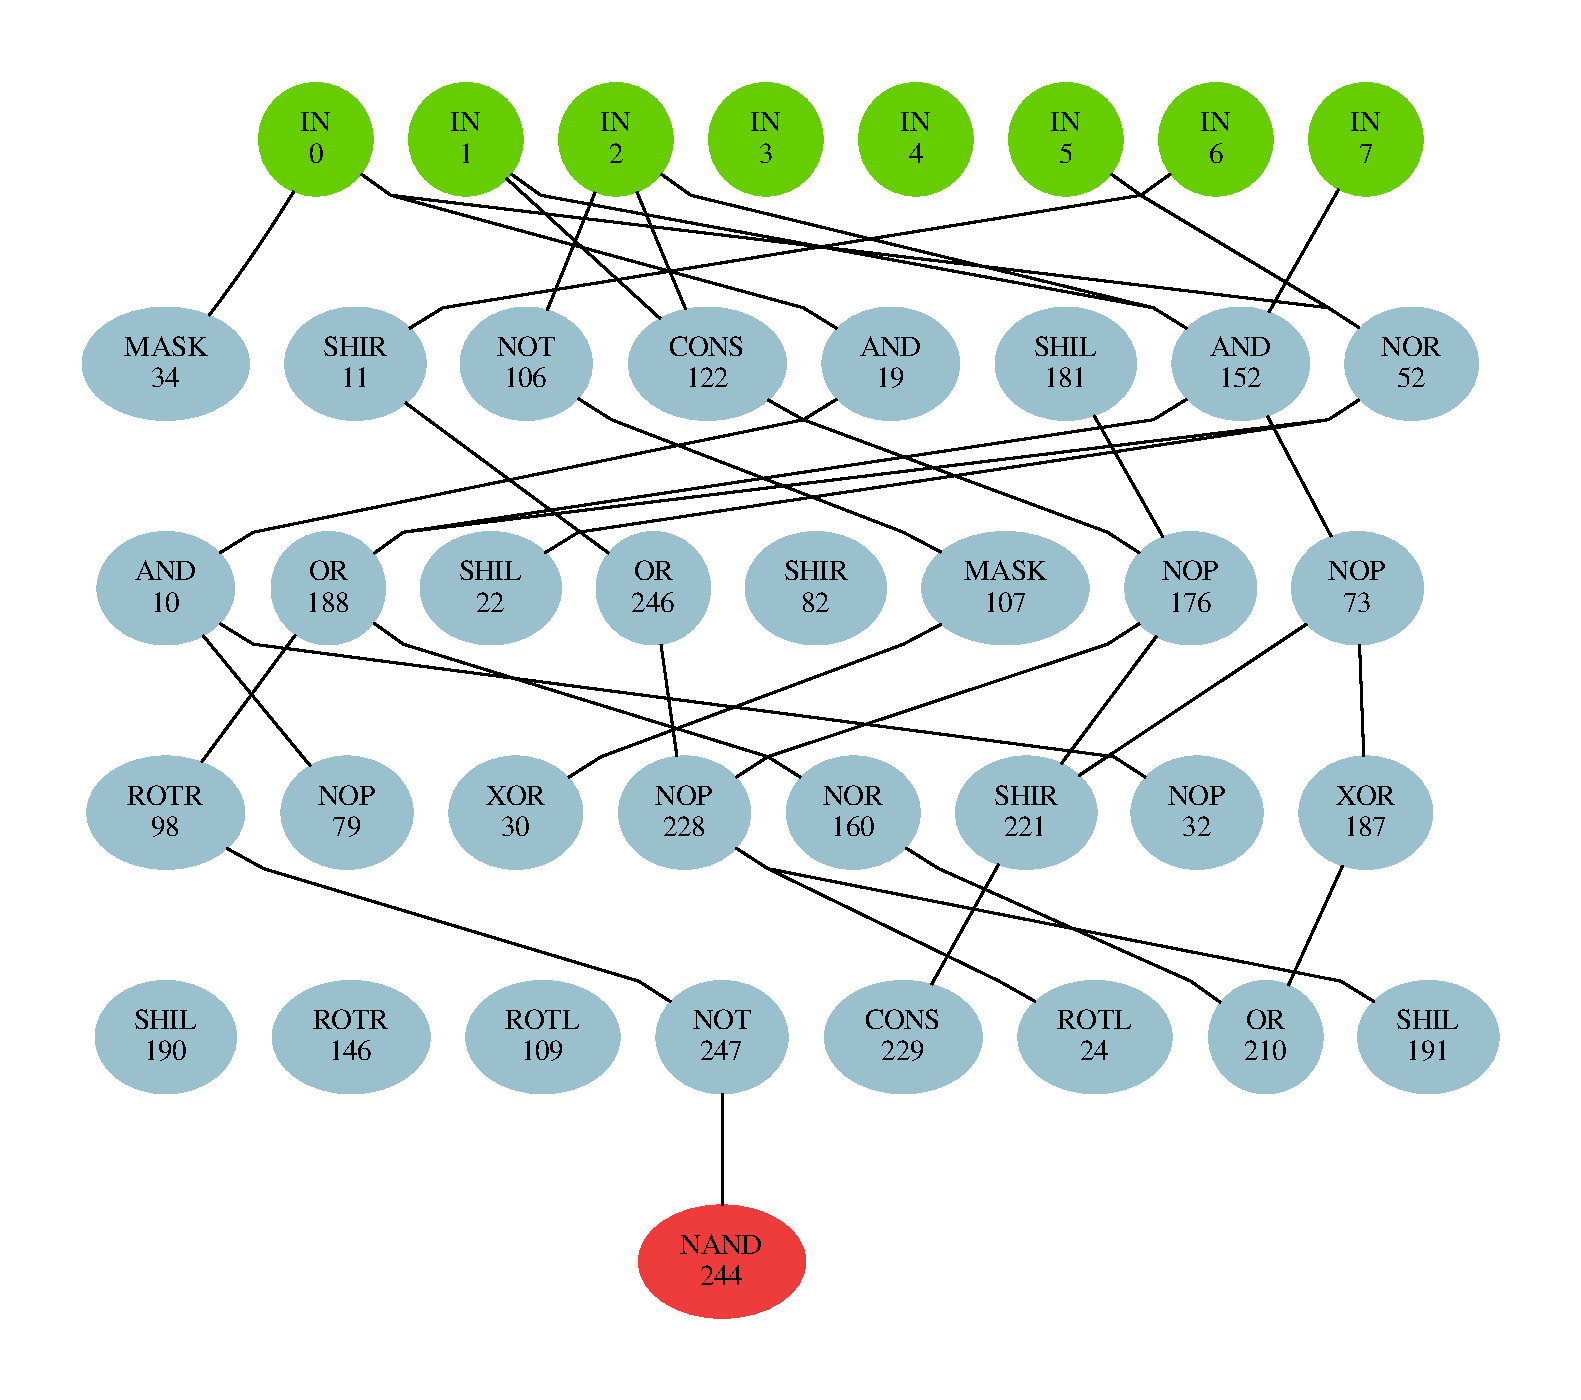
\includegraphics[width=0.9\textwidth]{./graphics/gls/circuit}
\caption{The distinguisher circuit representing a \textit{candidate solution} in EACirc computation. The red layer consists of input nodes, blue are internal nodes that transform the data and the red node is output node.}
\label{fig:eac-circuit}
\end{figure}

The distinguisher is not able to classify a single test vector, as it is possible even a truly random test vector may look like the tested data. Therefore, EACirc process the output statistically. It proceeds 1\,000 analysed data test vectors and 1\,000 reference random data vectors, and it accumulates the outputs per dataset to output distribution. These distributions for tested and reference datasets are compared using a $\chi^{2}$ test. The result of the $\chi^{2}$ test is a $p$-value, which is transformed to the \textit{fitness} value as $1 - p$-value.

There is an enormous number of potential circuits. Therefore the computation starts with a randomly generated circuit, generally denoted as \textit{candidate solution}. To obtain intended solution, we perform modifications, whose are addition or removal of a connector or change of the operation in the node. By these changes that we denote \textit{mutation}, we can create another \textit{candidate solution}.

Those two \textit{candidate solutions} are compared using the \textit{fitness}. We want to minimise the $p$-value, which means maximise the \textit{fitness}. Therefore we select the \textit{candidate solutions} with higher \textit{fitness}. We repeat the process 100 times, these iterations are called \textit{epoch}.

At the end of the \textit{epoch}, there is a likelihood that the circuit exploited some property of the tested data. To not \textit{overfit} to the data, we change the tested datasets and repeat the \textit{epoch}.

This whole process is in terms of optimisation methods called \textit{iterated local search}. It is a metaheuristic from a list of single-solution metaheuristics.


\chapter{Metaheuristics}
\label{chap:metaheuristics}

A computational problem is a task to find a solution for given question. An optimisation problem is a task to find the feasible solution, which satisfies the criteria best. A heuristic is a problem specific technique for finding some approximative solution, where exact techniques fail. Finally, the metaheuristic is technique abstracted from the problem so that it can be used for various optimisation problems.

Metaheuristics are applicable for optimisation problems if a programmer can provide three crucial parts. First is an instance of candidate solution for the problem, it is the circuit in EACirc. Second is a function to vary the solution, in EACirc it is the mutation. Third and usually the most important is the fitness function, which measures the quality of the solution. Metaheuristic uses these parts to follow the landscape of the problem, and they try to find better solutions during the time.

The main advantage of metaheuristics is that they are well-known and studied. This overview, as well as implementation ideas, are following book Metaheuristics from Talbi~\cite{talbi2009metaheuristics}. Please refer to this book for more examples of metaheuristic applications, whose are out of the scope of this work. The citations that are mentioned in this thesis extend the literature of the book, mainly in areas close to application in cryptography.

The number of candidate solutions inspected simultaneously splits metaheuristics into two categories: single-solution metaheuristics are present in \cref{sec:opt-single-sol} and population-based metaheuristics in \cref{sec:opt-population}. \Cref{sec:opt-other} describes other methods. All the approaches are firstly described and then analysed for application in randomness testing. If the application is suitable, we describe more details about the possible implementation.


\section{Single-solution metaheuristics}
\label{sec:opt-single-sol}

\Cref{fig:opt-single-sol-overview} shows the classification of the improved variants of local search metaheuristics by authors of ParadisEO library.

\begin{figure}[H]
    \centering
    \footnotesize{
    \begin{tikzpicture}[->,>=stealth',level/.style={sibling distance = 7cm/#1,
        level distance = 1.5cm}, every node/.style = {shape=rectangle, 
        draw=white, align=center}]]
      \node {Strategies for improving local search}
        child { node [xshift=3 cm] {Iterate with different\\solutions} 
            child { node {Multi-start\\local search} }
            child { node [xshift=-0.8 cm] {Iterative local\\search, GRASP} }
        }
        child { node {Change landscape\\of the problem}
            child { node [yshift=-1.2 cm, xshift=-0.6 cm] {Change of the objective function\\or the input data}
                child { node {Guided\\local\\search} }
                child { node {Noisy method} }
                child { node {Smoothing\\method} } }
            child { node [yshift=-1.2 cm, xshift=0.6 cm]  {Use different\\neighbourhoods}
                child { node {Variable\\neighbourhood\\search} }
            } 
        }
        child { node [xshift=-3 cm] {Accept non-improving\\neighbours} 
            child { node [xshift=0.8 cm] {Simulated\\annealing} }
            child { node [xshift=-0.8 cm] {Tabu\\search} }
        };
    \end{tikzpicture}
    }
    \caption{Single-solution metaheuristics as specialized version of local search. The source:~\cite[Figure~2.24, p.~125]{talbi2009metaheuristics}.}
    \label{fig:opt-single-sol-overview}
\end{figure}

\subsection{Local search}
\label{subsec:opt-single-sol-ls}

Local search is the very basic approach in problem optimisation. The search begins with a single candidate solution, and it applies changes to this solution forming neighbour candidate. Then the local search compares fitnesses of these two solutions and selects the better candidate to the next generation. The algorithm iterates this approach until it finds a satisfactory solution, or it ran the limited amount of iterations.

The algorithm can also be referred as hill-climbing, as we with acceptance of an improving solution, we step up in the fitness space. Therefore local search often finds only the sub-optimal solution -- a local optimum.

Escaping local optima is an important phenomenon, as fitness function landscape depends on tested data, or on the specific evaluation approach.

As EACirc is using an iterated version of local search, the application of local search would be straightforward. However, this would decrease the capabilities of EACirc do to omit of the learning process.

\subsection{Iterative local search}
\label{subsec:opt-single-sol-ils}

Iterative local search is and extension of local search. After defined amounts of iteration of basic local search, the tested data are changed. The computation on one set of data is called an \textit{epoch}, and the amount of iteration is called \textit{epoch length}.

During the \textit{epoch}, the fitness progress is non-decreasing. However, after the end of each \textit{epoch}, the fitness is expected to drop. The final fitness has to be tested on a new dataset, which applies for every metaheuristic. Therefore, we distinguish between the learning dataset and the testing dataset.

The \textit{epoch length} is the crucial parameter of this metaheuristic. A short epoch length can be computationally more demanding due to higher data consumption, and the solution may not be able to learn anything on the data. Too long \textit{epoch} leads to \textit{overfitting}, a situation when the individual is learning a specific pattern of the current dataset over general patterns of all datasets. Martin Ukrop examined the overfitting process in EACirc in~\cite[Chapter~7]{ukropBcThesis}.

The EACirc have used the iterated local search since~\cite{sys2014constructing}. Therefore it is used as a baseline for single-solution metaheuristics tested in this work.

\subsection{GRASP}
\label{subsec:opt-single-sol-grasp}

The greedy randomised adaptive search procedure is splitting each iteration into two steps: a feasible solution construction by greedy algorithm and performing the local search using the generated solution.

We abandoned this metaheuristic as we did not found any greedy algorithm for circuit construction, such that would reflect tested data. Also, it does not fit the iterative process of learning in \textit{epochs}.

\subsection{Multi-start local search}
\label{subsec:opt-single-sol-msls}

Multi-start local search is another approach how to surpass local optimum to find the global optimum. The metaheuristic starts the computation with $k$ randomly generated individuals that are concurrently optimised by local search.

This parallelism could increase the usage of the testing data in EACirc. The disadvantage is a more difficult evaluation, as Ukrop stated in~\cite[Chapter~5]{ukropBcThesis}. It is a question if we should evaluate the best, the average, or a random solution, or more solution simultaneously. Another possible advantage of multi-start local search can be parallelization of the computation. However, EACirc computation is already parallelized, neither on the level of single computation. Due to statistical interpretation, we have to repeat the computation process 1\,000 times.

We decided not to cover multi-start local search, as saving a small fraction of computation time for more complicated interpretation is a bad trade-off.

\subsection{Guided local search}
\label{subsec:opt-single-sol-gls}

Guided local search is metaheuristic based on dynamic changing of the fitness function. If the metaheuristic got stuck in local optima, guided local search would change the fitness function so the individual can continue climbing.

The EACirc computation can get trapped in a local optimum mainly in two cases:

\begin{enumerate}[noitemsep,topsep=3pt,parsep=3pt,partopsep=3pt]
    \item the individual got lucky to guess current test set, but it will not be successful in next \textit{epoch}, or
    \item the individual is already successful due to finding feature of the tested data, but it could not get better.
\end{enumerate}

We do not need to fix the first case, as such individual would be replaced in next \textit{epoch}. However, we can use guided local search to improve individual from the second case. Our alternative fitness function can be designed as the sum of our current fitness and e.g. the number of connectors. Such fitness would simplify the solution, which would help us with the interpretation of the last individual. Alternatively, we can use completely different fitness function.

We decided to implement guided local search in EACirc, as it also represents single-solution metaheuristics with a change of the objective function from \cref{fig:opt-single-sol-overview}.

\subsection{Noisy method}
\label{subsec:opt-single-sol-nois}

The noisy method is another metaheuristic, which changes the fitness space to escape local optima. It is done by adding random noise to the input data, as Talbi described in~\cite[Section 2.9.2]{talbi2009metaheuristics}. At the beginning of the computation, the noise is the strongest, and it disappears during the computation, so the final \textit{epochs} can be evaluated on the original data.

In EACirc, our research goal is already distinguishing pseudo-random data from truly random data. An additional random noise in the input would probably lead to an even more complicated learning process. For example, the noise could flip a bit on a position, which is necessary for distinguishing between the data sources. Therefore was this method abandoned.

\subsection{Smoothing method}
\label{subsec:opt-single-sol-smooth}

Smoothing method is the another metaheuristic, which uses changes in fitness function to escape local optima. The method is based on smoothing the landscape of fitness function by computing a local average of all neighbours to given distance. If the fitness is overall increasing in one direction, but more zoomed observation shows small fluctuation, smoothing method smooths the fluctuation and allows locating the global optima.

\textit{Neigbours} in EACirc are defined as solutions obtained by mutation of the circuit. Available mutations are connecting or disconnecting a connector, or change of the Boolean function in the node. The neighbourhood of an individual in EACirc is enormous (over $2^{25}$ neighbours in the distance one for the basic EACirc setup), this method would not be possible due to computational requirements.

\subsection{Variable neighbourhood search}
\label{subsec:opt-single-sol-vns}

Variable neighbourhood search also changes the landscape of the problem. However, it does not modify the fitness function or its interpretation, but it defines other methods for neighbour selection. If the computation gets trapped in local optima, the neighbourhood method is changed. Alternatively, the neighbourhood can be changed periodically. This method does not guarantee to escape from local optima, as all neighbourhoods can contain only worse solutions.

Specifying different neighbourhood in EACirc is hard. However, the method lead us to a different idea. EACirc is heading two mutually exclusive problems. We would like to have circuit connected sparsely for easier interpretation of the final solution. However, we also want to have the circuit's input and output nodes connected. We can solve the problems by reduction of the searched neighbourhood.

If we already have a successful solution, we can inspect only solutions with fewer connectors. In contrast, if the circuit is not connected (therefore the circuit's fitness is equal to zero), we can inspect only the individual with more connectors.

\subsection{Simulated annealing}
\label{subsec:opt-single-sol-sa}

Remaining two single-solution metaheuristics can accept non-improving neighbours. Short term acceptance of worse solution can lead to escape from local optima and finding global optima in whole computation.

Simulated annealing metaheuristic is inspired by the physical process of annealing in metallurgy. The annealing is an iterative process of heating the metal to increase the size of the crystals, which reduces the probability of a defect. During the process, the metal is heated to lower and lower temperatures.

Simulated annealing uses variable temperature, which describes the probability of acceptance of worse neighbour. This probability is decreasing during the computations, such that in the beginning, the likelihood of acceptance of worse solution is high, but at the end of the computation, only better solutions are accepted.

This metaheuristic is widely used, which was the reason for implementing it as a testing scenario for metaheuristics. Besides, it serves as a represent of the group of single-solution metaheuristics that accepts non-improving solutions. Its implementation in EACirc does not require complex changes, only the specification of this method. However, this method is not specified for the iterative approach with learning \textit{epochs}.

\subsection{Tabu search}
\label{subsec:opt-single-sol-tabu}

Similarly to simulated annealing, tabu search can also accept non-improving solutions to escape from local optima. However, the decision whether to accept a non-improving solution is not stochastic, but it is based on knowledge of already visited solutions. Therefore, tabu search holds a memory of visited solutions, called \textit{tabu list}, and it would not use twice the same solution. This way, tabu search avoids cycles during the optimisation process.

Application of tabu search in EACirc has several issues. Firstly, how to store used individuals (memory usage may be a problem), which can be solved by storing only a hash of the solution. Secondly, the neighbourhood space of an individual is huge, as stated in \cref{subsec:opt-single-sol-smooth}. It is higher than the number of individuals tested during whole computation. Choosing twice the same solution is unlikely. Therefore we decided to try only simulated annealing and leave the decision of tabu search implementation on the result of simulated annealing.

\section{Population-based metaheuristics}
\label{sec:opt-population}

Population-based metaheuristics are usually inspired by biological processes. The group of evolutionary algorithms is motivated by the process of biological evolution, which treats a population of species and forms better individuals. The ant colony optimisation and swarm intelligence algorithms are based on motion behaviour of a colony of selected species.

Population-based metaheuristics are usually more complex than single-solu\-tion metaheuristics. The complexity occurs on multiple levels.

\begin{itemize}
    \item The implementation usually requires many configurable parameters; therefore it is more prone to programming mistakes.
    \item The fine-tuning of these parameters can be sensitive to the selected problem.
    \item The algorithm needs more computational resources due to overhead with maintenance more complex method.
\end{itemize}

However, population-based metaheuristics bring significant advantage. The population together may prevent the algorithm from ending in local optima, as long as the metaheuristic maintains well the diversity of the population.

\subsection{Evolutionary algorithms}
\label{subsec:opt-popul-ea}

Evolutionary algorithms are a group of population-based metaheuristics inspired by the natural selection in the evolution of the species. They are the most spread and studied population-based metaheuristic, in computer science since the 1980s. Evolutionary algorithms can be used to solve both continuous and discrete problems, and they are also used for both single- and multi-objective problems.

The computation is an iterative loop of three main steps, together denoted as a generation. The evolution starts with a random population of initial solutions.

\begin{description}
    \item[Selection of parents] from the population. Usually based on the fitness function with some randomization technique.
    \item[Reproduction to new offsprings] using mutation and crossover -- an algorithm for recombination of two parents. 
    \item[Population replacement] by offsprings. Here can be again used the evaluation by fitness. 
\end{description}

This iterative approach can by usage of well-selected fitness, mutation and crossover increase the quality of the individual. The algorithm can be stopped by the number of generations or by achieving target fitness.

During the 40 years, many variants of evolutionary algorithms emerged.

\begin{description}
    \item[Genetic algorithms] traditionally use bit representation of the individuals. It applies both mutation and crossover to create new individuals. The selection of new population from the offsprings is stochastic.
    \item[Evolutions strategies] are used in continuous optimisation, so the individuals are represented by real values. The main way of creation new offsprings is the mutation; the crossover is rarely used. They apply elitist selection to form a new population.
    \item[Evolutionary programming] is used in series prediction problems and continuous optimisation. It emphasises mutation and does not use recombination. The population is selected stochastically.
    \item[Genetic programming] evolves programs as solutions. They are usually expressed as a tree (like abstract syntax tree). Both mutation and crossover are applied. Even though genetic programming is the least studied approach of evolutionary algorithms, and it is computationally expensive, it is used in classification problems.
\end{description}

Randomness testing is a discrete optimisation problem; therefore we may apply genetic algorithms and genetic programming. Genetic algorithms were used in multiple works for analysis of bias in ciphertext from round reduced TEA and DES functions~\cite{twoRoundsTea,fourRoundsTea,fiveRoundsTea,song2007cryptanalysis,husein2007genetic}. On the other side, we found no successful work on the same topic using genetic programming.


\subsection{Ant colony optimization}
\label{subsec:opt-popul-aco}

The ant colony optimisation is an instance of swarm intelligence metaheuristics. This metaheuristic imitates the cooperative behaviour of ants. Every ant has a simple goal of collecting food, and the common goal is to find shorted path between the food and the nest. The motion of the ants is coordinated by their smell and a pheromone.

\begin{itemize}
    \item Every ant spreads pheromone on its trail.
    \item Ant prefers to take a path with more pheromone.
    \item The pheromone evaporates over time.
\end{itemize}

The common application of ant colony optimisation is on shortest path algorithms. The literature states many applications in travelling salesman problem~\cite{dorigo1997ant}. However, the metaheuristic can also be applied to combinatorial problems, as the problem representation can be encoded to the graph structure and the shorted path algorithm may solve them. An example of such application can be formula satisfiability problem (SAT)~\cite{moritz2010solving}.

The problems solvable by ant colony optimisation are usually problems, where the solution is constructed from building blocks. The pheromone can be associated with the block, and it can describe the probability of using the block in the final solution. However, EACirc's circuit cannot be decomposed into independent components, so we do not test this metaheuristic.

\subsection{Scatter search}
\label{subsec:opt-popul-scatter}

The scatter search method is highly utilising the combination of the individuals. The algorithm holds a population of the best so far inspected individuals called \textit{reference set}. Like every population-based metaheuristic, the diversity of the \textit{reference set} is crucial. Scatter search is an iterative algorithm, where one iteration consists of 4 steps.

\begin{enumerate}
    \item The \textit{reference set} is split to a subset of size 2 to 4 individuals.
    \item We combine the individuals of the subsets to create new candidate individuals.
    \item We run a single-solution metaheuristic to improve the candidate individuals.
    \item The \textit{reference set} incorporates the candidate individuals based on fitness.
\end{enumerate}

The main problem of application is the second step, where are solutions combined. We would have to develop a function, which combines multiple solutions and takes their shared properties. However, there is no guarantee that various advanced individuals share the same property. Also, the approach is similar to evolutionary algorithms. Therefore we did not test it.

\subsection{Other swarm intelligence methods}
\label{subsec:opt-popul-si}

The swarm intelligence metaheuristics adopt a collective behaviour of decentralised and self-organized systems. Similarly to ant colony optimisation, the behaviour of the swarm can be used to solve optimisation problems. Usually, the best application is in problems that are close to the origin of the behaviour of the swarm. Therefore, the main application is in decentralised control of robots, droids and other artificial individuals.

The application issues for our problem are similar as for ant colony optimisation.

\section{Other methods}
\label{sec:opt-other}

There are various optimisation methods, which are not classified as single-solution or population-based metaheuristics. However, those models or algorithms are still capable of learning of classification.

The classification is important in machine learning area. Therefore, the following models have developed advanced methods not only to the process of learning but also the interpretation of the results, detection of outliers, learning on a low amount of data or non-complete data. Because of these advantages, we decided to experiment with them.

These models and algorithms can be used for various goals. Two main are feature selection and classification. Our principal aim is the classification, while we expect, that the model itself will select the features. The model has to adapt to the data. Therefore we cannot make manual feature selection.

% what ML problem specification heads-to?
% ML is well studied, but the main problem is selection of the method, fine-tuning the parameters and setting up the features

\subsection{Artificial neural networks}
\label{subsec:opt-other-ann}

The artificial neural networks (ANN) are classification optimisation method inspired by the process of learning of brain and neural system. The initial idea was inspired by the research of Donald Hebb~\cite{hebb49learning}, who described the neurones and the process of learning of living beings neural systems. The Hebbian learning arose several trivial nonsupervised learning methods. Further development came with the invention of backpropagation algorithm by Paul Werbos~\cite{werbos75beyondThesis}. The last rapid increase of usability of artificial neural networks came in 2006 with significant speed-up both of algorithm and its application on GPUs, which allowed deeper networks and more analysed data due to parallelization, leading to rapid progress in scalability and usability of artificial neural networks.
% deeper introduction to ANN can be found in book http://www.deeplearningbook.org

The artificial neural network consists of purpose specialised layers. The first layer is called visible layer, and its input is the data for classification. Then there may be many hidden layers, which sequentially process the output of previous layers. The data proceed to the last -- output layer, which decides the classification. Each layer consists of neurones. Each neurone takes as input the output from all neurones of previous layers, and weight for each connection multiplies these outputs. The output is processed by an activation function, which ensures normalisation of the output. There are many types of activation function, and each layer can use different activation function. The most used activation function is a sigmoid function, with input from real number and output is usually from the interval $(-1, 1)$ or $(0, 1)$.

%\todo{citations: }
The artificial neural networks were used to solve various problems in classification and pattern recognition. The most common are applications in image processing, signal processing, text data processing and in robotics and system control.

In cryptography, we have seen fewer applications of ANN. The main area of application of ANN in cryptography is authentication~\cite{li2001remote}, as it is a classification problem, where learning methods can bring speed-up traded off by approximation that allows errors.

Application in encryption is even rarer. For example, researchers from Google Brain showed an experiment where they let neural network develop encryption function for communication, while another neural network was intercepting the communication and attempting to decrypt it~\cite{abadi2016learning}. Preceding works~\cite{shihab2006backpropagation, volna2012cryptography} did not get such attention as Google's work, but they had a similar objective with simpler assumptions. However, all these works are far from application in cryptography. The only inspiration from them to our project is normalisation of binary data to floats, that was done by encoding zero as $-0.5$ and one as $+0.5$. We have found no further relevant application of ANN in the classification of binary data.

We would like to utilise the developed approach of learning in classification by ANN. However, the application of ANN in our scope is not straightforward. We do not know in advance, what are the features in the data. Therefore the network has to have the whole ciphertext as an input. We encode the binary input to floats (0 as $-0.5$ and 1 as $+0.5$) based on intuition supported by other works~\cite{abadi2016learning,shihab2006backpropagation}. We tried both fully connected network (where every node is connected to every node of previous layer or every input bit), and convolution network, where the first layer has only a limited local interval of inputs. 


\subsection{Other statistical classification methods}

There are several other models or algorithms of statistical classification. Those are for example support vector machine (SVM), decision tree with a C4.5 algorithm, $k$-nearest neighbours algorithm ($k$-NN), Bayes classifier and many others. Those methods usually rely on good feature selection, which we do not perform in our scenario. Therefore, the application of those models was not examined within this work, but they might be an interesting question for further works.

\chapter{Experiment methodology}
\label{chap:method}

The primary testing goal of EACirc is to assess randomness of ciphertext of cryptographic functions. As most of the cryptographic functions are in a scope of automated analysis semantic secure, EACirc can identify non-randomness only for reduced functions. The functions can be reduced in a number of rounds, by processing selected plaintexts, and by selecting only specific bits of the output. As the analysis of reduced versions of cryptographic functions is the main goal of the EACirc project, it is also selected as the testing scenario for comparison of analysed metaheuristics.

The approach for evaluation is briefly described in \cref{chap:eacirc}. The tested data were produced from 16 different cryptographic functions. These functions are reduced by the number of rounds. We selected intervals of rounds based on EACirc reference capabilities, such that the EACirc is capable of distinguishing function reduced to $i$ rounds, but it is not able to distinguish $i+1$ rounds\footnote{Further is this round setting referred as "an edge".}. Usually we test also $i-1$ and $i+2$ rounds, for broader comparison of the results with state of the art of cryptanalysis.

EACirc works as distinguisher between tested dataset (produced by the cryptographic function) and reference random data. Formerly we used quantum random number generator (QRNG) services as the source of this reference data. This have following disadvantages:

\begin{itemize}
    \item Need of having QRNG data for the computation.
    \item Potential of an error due to bad data. QRNG are not error less, for example, Quantis device we tested in our laboratory produced \href{http://rtt.ics.muni.cz/ViewResults/Experiment/1732/}{biased data}. Detection of such biases is common use-case of randomness testing.
\end{itemize}

Therefore we switched from QRNG to pseudo random number generator (PRNG) PCG32~\cite{pcgGen} as reference data. PCG32 is fast and computationally strong PRNG. We did experiment of comparison PCG32 with QRNG and we found no bias, as well as we retested old results using QRNG newly with PRNG and the results are the same. Hence, we believe build-in PRNG is a more secure and convenient option.

\section{Used data}
\label{sec:method-data}

Previous works on EACirc analysed candidates of cryptoprimitives competitions~\cite{estreamMgrThesis,sha3Thesis,ukropMgrThesis}. These works extended EACirc by many functions sharing the same interface. This approach was effective for broad analysis of the competition candidates, but it does not test well-known cryptographic functions like AES and DES.

Therefore, for the comparison with other randomness testing tools and other research papers on semantics security, we decided select new test set of cryptographic functions. We chose the finalist of competitions SHA-3 (BLAKE, Gr\o stl, JH, Keccak and Skein) and eSTREAM (HC-128, Rabbit, Salsa20, SOSEMANUK and Grain), and above that, we implemented other block (AES, DES, 3-DES and TEA) and stream (RC4) functions.

\subsection{Reimplementation of stream handling in EACirc}
\label{subsec:method-data-streams}

The implementation of SHA-3 and eStream candidates in EACirc was called \todo{projects}. The projects were handling everything related to data generation, specifically IV, key and plaintext. Every project had its own implementation of counter plaintext generator, strict avalanche criterion generator and so on.

For the implementation of the new project for block ciphers, we decided to reimplement data generation in more variable and modifiable way. For this, we decided for data manipulation via streams, whose can be nested into each other. Each stream implements simple interface with constructor and function \texttt{next}, which returns next test vector. The stream is specified only by the output size of the test vector.

The purpose of stream is unification of all data manipulation in the whole project, independently on the used cryptographic function. All streams inherit from abstract class \texttt{stream} with minimalistic interface. The streams have to specify its \texttt{size} and they have to implement method \texttt{next()}, which returns next test vector. We have currently many types of streams in EACirc.

\begin{itemize}
    \item Data sources streams, that are used as an input to cryptographic functions or as reference data. Example of such streams are:
    \begin{itemize}
        \item input streams: true and false bits generators, counter and multiple variants of the strict avalanche criterion generator, and
        \item PRNG's PCG32~\cite{pcgGen} and Mersenne Twister~\cite{matsumoto1998mersenne}.
    \end{itemize}
    \item Projects of cryptographic functions. Namely project eSTREAM and SHA-3.
    \item Postprocessing streams are applied to data from cryptographic functions for more advanced experiments. They allows us analysis of selected bits of the function.
\end{itemize}

The streams are completely configurable via \texttt{JSON} configuration file. As the streams can be nested, the structure is described as a \texttt{JSON} tree. This updates changed the structure of the configuration file, therefore the configuration files are not backwards compatible. Nevertheless, the configuration is described and shown on examples in the project's documentation~\cite{EACirc-wiki-streams}.

All these changes significantly simplified the codebase, unified many implementations of the same functionality and broadened the experiment capabilities of EACirc. Therefore it was the main feature for EACirc~4.1 release.

\subsection{Implementation of functions}
\label{subsec:method-data-funcs}

As the source of AES, DES and 3-DES implementations was used educative repository~\cite{cryptoFunc}. The author of this repository verifies the encryption to the test vectors to ensure correctly working implementation. The only modification of the code is a limitation of the functions in the number of rounds.

TEA implementation is based on Wikipedia code~\cite{teaWiki}, and it was already implemented in EACirc before. The implementation was simplified and reduced due to changes in the interface. It is also reduced to selected amount of rounds.

RC4 is also based on the educative repository~\cite{cryptoFunc}, but as RC4 has no round structure, therefore, the code is unchanged.

All these functions together with the new interface of new block project and test vectors processing algorithm were released in minor version EACirc 4.1.

\paragraph{Corrections and code review of SHA-3 and eSTREAM functions} was another part of streams update. Multiple cryptographic functions from previous implementation were incorrectly round-reduced.
\label{par:method-data-funcs-bugs}

\begin{itemize}
    \item SHA-3 Skein, eSTREAM Rabbit, SOSEMANUK and F-FCSR were not round-reduced, but their implementation uses iterative approach, so we reduced them.
    \item eSTREAM HC-128 stated in the project documentation and in header file, it can be round-reduced, but it had no effect in the core function at all.
    \item eSTREAM Salsa20 used wrong implicit number of rounds for default settings.
\end{itemize}

These bugfixes together with fix of improper configuration of eSTREAM project were one of two major reasons for releasing EACirc 4.2. All these fixes together with valid configurations are described in project documentation~\cite{EACirc-wiki-streams}.

\subsection{Data generator tool}
\label{subsec:method-data-generator}

For direct comparison of the tested methods, we need to analyse the same data. EACirc has build in generation of test vectors, to feed the computation, as is described in \cref{sec:method-data}. Therefore, we implemented side project from EACirc for production of data. We call it \textit{Generator} and it shares the source code of functions with EACirc. This is done using GitHub submodules, so the \textit{Generator} has its repository~\cite{EACircStreams}.

The \textit{Generator} is fully configurable via \texttt{JSON} configuration file as EACirc. The structure of the file is reduced, as the configuration describes only generated data. So the \textit{Generator} inherits all the capabilities of streams, providing complex control on the data production. For simplification and automation, we also prepared script, that generates configuration files for most common settings, which allows simple execution by command line arguments. For even simpler acces to testing data, we generated 160~MB file for each basic setup for each widely-known cryptographic function (described in \cref{subsec:method-data-funcs}) reduced to wide interval of rounds. This dataset is publicly accessible \href{https://drive.google.com/drive/folders/0B5Z1zst5NzwXQmFKaXgxREJWNk0?usp=sharing}{online}.

We have ongoing plan of publication, which will crucially utilize the \textit{Generator}. It will be paper on comparison of statistical testing tools on wide variety of cryptographic data. The \textit{Generator} will be used as it unifies many different cryptographic functions and it can reduce the functions in number of rounds, or selection of specified bits. The \textit{Generator} has already all the necessary features, so we can start with writing of the paper when we select the conference, we are aiming for.

Important work for the generator was fixing the implementation bugs, described in previous~\cref{par:method-data-funcs-bugs}.


\section{Methodology for specific optimisation methods}
\label{sec:method-spec}

As the tested scenarios vary not only by optimisation method but by used tools as well, the methodology changes for given metaheuristics. The base of the experiment was used for single-solution metaheuristics, as they were implemented directly to the EACirc and they inherited the experiment environment of our tool.

For direct inter-method comparison, we need to use the same data for testing. Therefore, all used data are generated from the same implementation, described in \cref{subsec:method-data-funcs}. The cross-method comparison is still sensitive to the testing approach, therefore we describe it in detail in following sections.


\subsection{Single-solution methodology}
\label{subsec:method-spec-ss}

All single-solution metaheuristics were implemented into EACirc, therefore they share the same computation and interpretation. The solution is represented as simulation of a circuit, described in the \cref{chap:eacirc}.

The main advantage of single-solution metaheuristics is their simplicity and straightforward interpretation. However, the overall interpretation of EACirc results became complex, as we work with randomness that needs to be evaluated statistically. The complex approach also leads to significantly better results. The statistical evaluation as well as distributed computation automation is described below.


\subsubsection{\textbf{Statistical evaluation}}
\label{subsubsec:method-spec-ss-stat}

\todo{ref to EAC chap}
The fitness of an individual is a $p$-value of two sample $\chi^{2}$ test, which tests, if the output bytes per source have same distribution. For a well-working individual on a weak source of data, the fitness is close to 1. As the quality of the individual decreases, the fitness decreases as well. However, completely random guess like coin tossing has the $p$-value uniformly distributed on the interval (0, 1).

As the $p$-values are uniformly distributed for random guess, getting high $p$-value can imply two cases. Either the $\chi^{2}$ test rejected the hypothesis and scored high confidential output, or the tested data, or in case of random guess, we were lucky and obtained high value from uniform ditribution on interval $(0, 1)$. Therefore, we avoid interpretation of a single $p$-value, we collect an $p$-value per every \textit{epoch}, and we process these $p$-values to Kolmogorov-Smirnov test. It analyses the uniformity of usually 300 $p$-values. This test is using significance level $\alpha = 1\,\%$, therefore it rejects the null hypothesis that tested data seems nonrandom in 1\,\% of runs. To avoid such case, we run the experiment with the same settings 1\,000 times and we analyse the \textit{rejection rate} given as the amount of failed KS tests per 1\,000 runs. If it is around 1\,\%, the data seem to be random, while in it is much higher, the experiment rejected randomness hypothesis of tested data.

This approach is vastly increasing the amount of data needed for the computation, as well as the overall run-time. This method is a trade-off for the success rate of EACirc, as different evaluators do not need statistical evaluation. Hence they need much fewer data; however, such evaluators are slightly worse based on the results from~\cite{svenda2013towards}.

When we consider basic setup for single-solution metaheuristics, EACirc consumes 4.8\,GB of ciphertext of tested function (\cref{fig:dataUsage}). The runtime of the experiment on MetaCentrum varies from 4 to 20 hours on a single core.

%http://tex.stackexchange.com/questions/57732/placing-figures-inside-a-two-column-document 3rd answer
\begin{figure*}[t]
    \begin{equation*}
        \begin{aligned}
    \Sigma = 1\,000 \;
             \frac{\textnormal{runs}}
                  {\textnormal{experiment}}
             \cdot
             \left(
             300 \;
             \frac{\textnormal{epochs}}
                  {\textnormal{run}}
             \cdot
             1\,000 \;
             \frac{\textnormal{vectors}}
                  {\textnormal{epoch}}
             \cdot
             16 \;
             \frac{\textnormal{bytes}}
                  {\textnormal{vector}}
             \right) \approx\\
             \approx 4.8 \textnormal{\,GiB per experiment}
        \end{aligned}
    \end{equation*}
    \caption{The amount of tested data analysed by EACirc for a single configuration of randomness testing experiment. A single run also evaluates randomness of the data, however the capability of EACirc decreases in such mode, and single result is prone to incorrect evaluation due to statistical error.}
    \label{fig:dataUsage}
\end{figure*}


\subsubsection{\textbf{Computation automisation}}
\label{subsubsec:method-spec-ss-auto}

As EACirc needs repeated computation on MetaCentrum grid infrastructure, the automation for binary deployment, computation distribution, aggregation of the results and their postprocessing are required.

The scripts are executed in few following steps.

\begin{enumerate}[noitemsep,topsep=3pt,parsep=3pt,partopsep=3pt]
 \item Firstly, a preprocessor creates necessary configuration files for the experiment.
 \item Secondly, MetaCentrum scripts distribute the computation among the grid infrastructure.
 \item Thirdly, after the computation finishes the postprocessor script aggregate the results. 
 \item Finally, the table generator script generates a human readable version of the results as well as database dump of the whole experiment. The whole process is shown in \cref{fig:scripts}.
\end{enumerate}

The EACirc project formelly used tool Oneclick created by Lubomír Obrátil~\cite{obratilBcThesis}. The Oneclick was a single tool for both preprocessing and postprocessing phase, and the run was parametrized. However, this approach was programmed for BOINC infrastracture and it is outdated for the MetaCentrum. The advantages of new scripts are: 

\begin{itemize}
    \item they are single purpose, easier to modify one without affecting other,
    \item they are written in bash (running scripts for MetaCentrum scheduler) and Python (processing), so they do not need to be compiled,
    \item they maintained up-to-date for the newest EACirc,
    \item they are faster, as MetaCentrum computation do not require formerly used redundancy procedures.
\end{itemize}

These scripts are expected to be modified by individual researchers for the needs of their experiments, so the scripts are stored in GitHub repository~\cite{eaUtils}, and users are supposed to fork them. The repository also contains \texttt{readme.md} file, with specifies the first steps with computations on MetaCentrum with these scripts. Every script then contains documentation in the code (concerning expected modifications for individual purposes), and when it is run without arguments, it prints out a help message.

\begin{figure}[H]
    \centering{}
    
\begin{changemargin}{-3cm}{-3cm}
    \centering{}
    \rotatebox{-90}{
    \scalebox{0.9}{
    \tikzstyle{block} = [draw, rectangle, minimum height=3em, minimum width=3em]
    \tikzstyle{el} = [draw, ellipse, minimum height=3em, minimum width=3em]
    \tikzstyle{cl} = [cloud, cloud puffs=10,cloud puff arc=120, minimum height=3em, minimum width=3em]
    \begin{tikzpicture}[>=stealth, auto, node distance=3cm, every text node part/.style={align=center}]
        \node [el] (e) [] {\bf{experiment idea}};
        \node [block] (pre) [below of = e,yshift=0.5cm] {\bf{preprocessor}};
        \node [block,text width=3.5cm] (run) [below of = pre,yshift=-0.5cm] {\vspace{0.1cm}{\bf runner scripts} \texttt{run\_experiment.sh} runs for every config file script \texttt{single\_job.sh}};
        \node [block] (eac) [below of = run] {\bf{EACirc}};
        \node [block] (pos) [below of = eac,yshift=0.6cm] {\bf{postprocessor}};
        \node [block] (gen) [below of = pos,yshift=0.6cm] {\bf{table generator}};
        \node [el] (res) [below of = gen,yshift=0.6cm] {\bf{readable results}};

        \draw [->] (e) -- node [right] {researcher modifies\\general setting} (pre);
        \draw [->] (pre) -- node [right] {produces config for\\all combinations\\of function and round} (run);
        \draw [->] (run) -- node [right] {distributes computations\\on MetaCentrum grid} (eac);
        \draw [->] (eac) -- node [right] {results are returned\\to the frontend server} (pos);
        \draw [->] (pos) -- node [right] {aggregates the results\\and computes the statistics} (gen);
        \draw [->] (gen) -- node [right] {generates human readable tables\\and dump the results} (res);
    \end{tikzpicture}
    }
    }
\end{changemargin}
    
    \caption{Execution of EACirc on MetaCentrum grid -- order and purpose of the scripts.}
    \label{fig:scripts}
\end{figure}

\paragraph{Preprocessor}

EACirc computation is based on a configuration file with specification and environment settings for particular experiment. As the test suite contains tens variations of parameters, it is necessary to automatize config file creation, so the user would not make a mistake during this process.

The scripts are written in Python and are maintained in variants per the scenario of tested functions.

\paragraph{Running scripts}

The scripts for distribution of computation among the MetaCentrum network are a result of Martin Ukrop's thesis~\cite{ukropMgrThesis}. They are continuously maintained in \texttt{EACirc-utils} repository~\cite{eaUtils} for current EACirc version.

As each experiment needs to be run multiple times for statistical evaluation, the scripts repeat the computation in a loop with different seeds usually for 1\,000 times. All runs are then collected by running scripts.

The current version of these scripts is also published on the GitHub~\cite{eaUtils}, and the forked repository is ready to run experiments in the usual way.

\paragraph{Postprocessor}

As the computations are repeated for statistical significance, the postprocessor script has to aggregate results from many produced files. It searches through output files and collects the results. Afterwards, it calculates an aggregated statistics of the experiment.

The output of the postprocessor is \texttt{JSON} dump of the results, whose are used both for human readable results generation and also storing the results for later usage.

\paragraph{Table generator}

The generator takes as an input the \texttt{JSON} dump of the results from the postprocessor. Currently, it only generates a \LaTeX table with highlighted results, but it can be extended for more complex manipulation with the results.

\subsubsection{\textbf{Goal specification}}
\label{subsubsec:method-spec-ss-goal}

\todo{Petr's comments are not corrected}

The ultimate goal of the experiments with metaheuristics is increasing detection capabilities of nonrandomness of tested datastream. For testing and measuring how a metaheuristic performs, we analyse swet of functions described in \cref{sec:method-data}. We increase the resolution of the comparison by testing cryptographic function reduced in number of rounds. However, reduction of the function to specific number of rounds is still a very steep, therefore the goal is hardly measurable on this scenario. The randomness of the data increases rapidly with the additional rounds of the cryptographic function. We would need functions with a low increase of entropy per round as a benchmark, but we did not observe such behaviour by any of the tested functions, nor our own design of benchmarking function do not behave that way~\cite{EACirc-lut}.

Less ambitious, but still useful goal can be an increase of the \textit{rejection rate} of the null hypothesis per experiment. Rejecting only 10\,\% of runs lead to difficulties with the analysis of the output test. The higher is the \textit{rejection rate}, the easier is the interpretation of found distinguisher. Also, if our \textit{rejection rate} is close to significance level $\alpha$, then the higher \textit{rejection rate} can overcome the edge value\footnote{For 1000 runs per experiment, this edge value is typically $2\cdot\alpha$. Such results can happen in less than 0.15\,\% of the experiments.} and we can reject the overall null hypothesis about the randomness of the source with higher confidentiality.

Another goal can be a decrease in the number of computations or the amount of used data. As we usually fix the epoch length to 100 iterations, the data usage and CPU time are directly related. Moreover, as the amount of used data is already high in this settings of EACirc, the time comparison is more valuable than consumed data comparison.

We can also analyse specific goals per metaheuristics. Both variable neighbourhood search and Guided local search set a complementary target in simplification of the circuits for later analysis. This goal is harder to measure, so the analysis is done less rigorously.

The EACirc project is using adaptive learning. During the computation, the tested data are changing. We analysed over-learning of the individuals during the learning process, and the over-learning can be analysed as well. Therefore, decrease over-learning can be another goal for metaheuristics.

\subsection{ANN methodology}
\label{subsubsec:method-spec-ms-aco}

The neural netowrk also classifies test vectors into 2 datasets -- the tested set and the reference set. Therefore, the implementation of takes as input 2 binary files -- a tested file and reference file. We generate these files with the \textit{Generator}, so we ensure consistency and comparability of the results within approaches. The results are concretely for the \href{https://drive.google.com/drive/folders/0B5Z1zst5NzwXQmFKaXgxREJWNk0?usp=sharing}{published dataset}.

The execution of neural network consist of training phase, where we iteratively provide different learning batches of data, and evaluation phase, where we use fresh data for final evaluation of ratio of correctly classified test vectors. The whole computation needs significantly less input data than EACirc, as is shown in \cref{fig:ann-dataUsage}.

\begin{figure*}[t]
    \begin{equation*}
        \begin{aligned}
    \Sigma = 
             100 \;
             \frac{\textnormal{epochs}}
                  {\textnormal{experiment}}
             \cdot
             25 \;
             \frac{\textnormal{vectors}}
                  {\textnormal{epoch}}
             \cdot
             16 \;
             \frac{\textnormal{bytes}}
                  {\textnormal{vector}}
             %\approx\\
             \approx {40 \textnormal{\,kB for learning +} \atop {40 \textnormal{\,kB for evaluation}}}
        \end{aligned}
    \end{equation*}
    \caption{The amount of data analysed by neural network for a single configuration of randomness testing experiment.}
    \label{fig:ann-dataUsage}
\end{figure*}

We prepared automation scripts for easier analysis of multiple files together. We have script for sequential execution of all the runs for all binary files in directory, which produces \texttt{JSON} results file. This file is afterwards proceed by script, which plots the learning progress and final correct classification ratio.


\chapter{Results}
\label{chap:res}

% TODO strange introduction, but we want this information somewhere
To verify every implemented method, we perform a \textit{sanity experiment} comparing random data to random data. Such a test gives us a reference \textit{critical value}, under which we do not reject randomness hypothesis. As this reference \textit{critical value} depends on the analysed method, we state it explicitly with every test scenario.

In \cref{sec:res-ss} we show results of single-solution metaheuristics, followed by \cref{sec:res-circ-anal} with analysis of metaheuristics influence on the complexity of produced distinguisher circuit. In \cref{sec:res-ann} we show results of ANN and finally in \cref{sec:res-comp} we compare all methods introduced in this thesis.

% SS methodology ref
\section{Single-solution metaheuristics}
\label{sec:res-ss}

%http://stattrek.com/online-calculator/binomial.aspx
\todo{this was already in previous chapter}
Single-solutions metaheuristics use evaluation described in \cref{subsubsec:method-spec-ss-stat}. It means, we execute EACirc 1\,000 times independently with the same setting and we evaluate how many of the runs rejected the randomness hypothesis. The number of rejections divided by the number of runs is called the \textit{rejection rate}. As we use a significance level $\alpha=1\,\%$, the \textit{sanity experiment} should reject the randomness hypothesis on average in $1\,\%$ of the runs. As we would like to have higher confidence in this \textit{sanity experiment}, we perform it with 100\,000 runs. The probability of incorrect \textit{rejection rate} of such case can be computed from the binomial distribution. For example, a \textit{rejection rate} higher or equal to $1.2\,\%$ of the \textit{sanity experiment} with 1\,000 runs can occur with probability of 4.787\,\%, while the probability decreases to less than 0.001\,\% for 100\,000 runs. We include the measured \textit{rejection rate} to the first row of further presented result tables. Other rows contain results of round-reduced cryptographical functions.

\Cref{table:res-usable-ils} and additional \cref{table:res-usable-sa,table:res-usable-gls,table:res-usable-vns} in the Appendix summarise results of the tested single-solution metaheuristics applied in EACirc. Every row of the table corresponds to one cryptographical function. The lower index after the function name specifies the number of rounds we limit the functions to in EACirc. The columns with -1, 0, +1 and +2 denote an offset to the number of rounds specified in the index. For example, AES$_{3}$ was tested reduced to two rounds, three rounds as default and four rounds. Five rounds were not tested, which is denoted by a dash in the corresponding cell. The number in the cell represents the \textit{rejection rate} for the particular case. For indistinguishable data, values around the \textit{rejection rate} of the \textit{sanity experiment} are expected. Results higher than twice the \textit{rejection rate} of the \textit{sanity experiment} can happen in less then 0.15\,\% cases for indistinguishable data, we denote it \textit{empirical critical value}. Therefore, results over the \textit{empirical critical value} are not considered random.

We use colours to ease the comprehension. Red highlight denotes that EACirc detected non-randomness. Green highlight signals that EACirc has not found any evidence against the randomness of the tested data. Therefore, we cannot say anything about the randomness of the data (we can neither reject, nor accept their randomness hypothesis). We highlighted untested scenarios (dash in the cell) if the results were estimated from prior works~\cite{svenda2013towards,sys2014constructing,kubicek2016new,ukropBcThesis} or faster test by statistical batteries. All the functions behave as expected; their randomness never decreases with an increasing number of rounds.

\subsection{Iterated local search}
\label{subsec:res-ss-ils}

As was stated in \cref{chap:eacirc}, EACirc used iterative local search as the metaheuristic since version 4.0. Therefore, measuring this metaheuristic serves as a baseline, which allows direct comparison of other metaheuristics. In addition, it can be used to estimate comparison to prior EACirc results~\cite{svenda2013towards,sys2014constructing,kubicek2016new,ukropBcThesis}, which were verified by this work.

\begin{table}[t]
\centering
\begin{tabular}{l|l l l l}
Function\textbackslash{}rounds & -1 & 0 & 1 & 2\\ \hline
rnd\_rnd$_{\textnormal{no rounds}}$ & --  & \fn{}0.01128& --   & -- \\\\
AES$_{3}$        & \fd{}1.0   & \fd{}0.160 & \fn{}0.007 & \fn{}--   \\
BLAKE$_{1}$      & \fd{}1.0   & \fd{}0.110 & \fn{}0.021 & \fn{}0.006\\
Grain$_{2}$      & \fd{}--    & \fd{}1.0   & \fn{}0.009 & \fn{}0.011\\
Gr\o stl$_{2}$   & \fd{}--    & \fd{}1.0   & \fn{}0.010 & \fn{}0.010\\
HC-128$_{\textnormal{no rounds}}$& -- & \fn{}0.008 & -- & --        \\
JH$_{6}$         & \fd{}--    & \fd{}1.0   & \fn{}0.012 & \fn{}0.008\\
Keccak$_{3}$     & \fd{}1.0   & \fn{}0.017 & \fn{}0.008 & \fn{}--   \\
MD6$_{8}$        & \fd{}--    & \fd{}0.774 & \fn{}0.008 & \fn{}0.011\\
Rabbit$_{0}$     &      --    & \fn{}0.017 & \fn{}0.007 & \fn{}0.015\\
RC4$_{\textnormal{no rounds}}$& -- & \fn{}0.011 & --    & --        \\
Salsa20$_{2}$    & \fd{}--    & \fd{}1.0   & \fn{}0.010 & \fn{}0.008\\
SINGLE-DES$_{4}$ & \fd{}1.0   & \fd{}0.204 & \fn{}0.001 & \fn{}0.010\\
Skein$_{3}$      & \fd{}1.0   & \fd{}1.0   & \fn{}0.016 & \fn{}0.010\\
SOSEMANUK$_{4}$  & \fd{}--    & \fd{}1.0   & \fn{}0.017 & \fn{}0.011\\
TEA$_{4}$        & \fd{}1.0   & \fd{}0.444 & \fn{}0.012 & \fn{}0.013\\
TRIPLE-DES$_{2}$ & \fd{}--    & \fd{}1.0   & \fn{}0.006 & \fn{}0.007
\end{tabular}
\caption{Results of iterated local search as EACirc metaheuristics on the well-known cryptographic functions. The values in the cells are the \textit{rejection rate} of the randomness hypothesis. The structure and the values in this table are explained in the \cref{sec:res-ss}.}
\label{table:res-usable-ils}
\end{table}

The results of iterated local search are shown in \cref{table:res-usable-ils}. From these results, we can conclude the following regarding the testbed.

\begin{itemize}
    \item The \textit{empirical critical value} (the result in the first row) is significantly (as is computed in \cref{sec:res-ss}) higher than 1\,\%. It is caused by a known, but yet an unresolved bug, described in the documentation~\cite{EACirc-wiki-bug}. This bug is a consequence of unconnected input to output in the circuit, so we denote it as the \textit{connection bug}. We tried fixing the \textit{connection bug} using many techniques. However, none of them was statistically sound, and none has fixed the issue globally.
    \item The randomness of three-round AES, one-round BLAKE, eight-round MD6, four-round DES, and four-round TEA is in the interpretation described in \cref{subsec:method-spec-ss} rejected. However, the \textit{rejection rate} is less than 100\,\%. Therefore, the probability of obtaining a working distinguisher is lower than 100\,\%. We denote these results as \textit{benchmarking functions} results, as the quality of different metaheuristics directly affect them. Therefore, these \textit{benchmarking functions} provide a highly sensitive comparison of the metaheuristics.
\end{itemize}

We also performed other tests, which showed some additional information.

\begin{itemize}
    \item It is possible to obtain the \textit{rejection rate} higher (up to full 100\,\%) than shows the \cref{table:res-usable-ils} for the \textit{benchmarking functions}. However, advancing the results require time-consuming manual fine-tuning to the tested data or more computational time. In the study of TEA~\cite{kubicek2016new}, we showed almost 100\,\% distinguisher for four rounds TEA. Obtaining such result required different shape of the circuit due to TEA block length and 100 times more test vectors. On the other hand, an increase of the \textit{rejection rate} by better metaheuristic applies in general, so all results should benefit such improvements.
    
    \item The results shown in \cref{table:res-usable-ils} were tested with the \textit{epoch length} of 100 generations. It means that the metaheuristic performed 100 generations on the same dataset. This setup seems to lead to overfitting, as Ukrop examined in~\cite[Section~7.1]{ukropBcThesis}. We tried decreasing the epoch length to 20, which lead to the increase of influence of the \textit{connection bug}, as the \textit{empirical critical value} raised to $0.03127$. Such setup did not increase the number of distinguished rounds for any function, but it increased the \textit{rejection rate} of all the \textit{benchmarking functions}. However, only the \textit{rejection rate} of three-round AES increased significantly to $0.982$. The same behaviour appeared for shorter epochs for all metaheuristics.
\end{itemize}

\subsection{Simulated annealing}
\label{subsec:res-ss-sa}

We tested the simulated annealing as a representative of single-solution metaheuristics that can accept a non-improving solution. The results are available in the Appendix as \cref{table:res-usable-sa}, as they are very similar to the \cref{table:res-usable-ils} with iterative local search results. A direct comparison of notable metaheuristics results on the \textit{benchmarking functions} will be summarised in \cref{sec:res-comp}.

The \textit{sanity experiment} ended with the \textit{rejection rate} of $0.01681$, which corresponds to a higher influence of the \textit{connection bug} for metaheuristics that accepts non-improving neighbour. As the \textit{rejection rate} of the random-random experiment increases, all other \textit{rejection rates} increase as well. Therefore, the \textit{connection bug} probably influenced \textit{benchmarking functions} results, so the increased \textit{rejection rate} of them may not imply a significant improvement.

The simulated annealing uses two configurable variables that influence the learning process. Those are the initial temperature and the cooling ratio. They both corresponds to the probability of accepting a non-improving solution. We analysed three different cooling scenarios, every on three different initial temperatures and cooling ratios. The cooling scenarios are illustrated in \cref{fig:sa-cooling-scenarios} and the difference is based on the behaviour on changed learning data. The tested variables were $(\mathit{initial~temperature, cooling~ratio}) \in \{ (500, 0.9), (100, 0.98), (50, 0.995) \}$. Every combination of cooling scenarios and temperature variables were analysed. The \cref{table:res-usable-sa} is the final and the best result of those nine tested configurations. The configuration is described by the blue temperature scheduling curve with the $\mathit{initial~temperature} = 500$ and the $\mathit{cooling~ratio} = 0.9$, as suggests Talbi in~\cite{talbi2009metaheuristics}.

\begin{figure}
\centering
    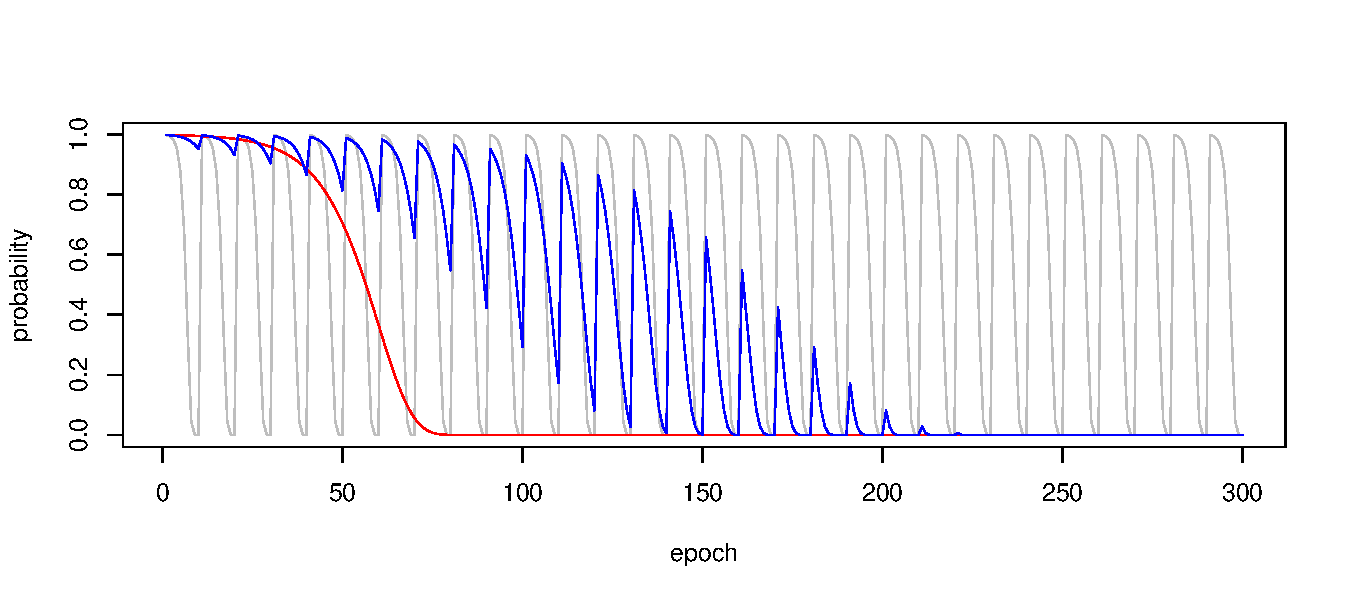
\includegraphics[width=\textwidth]{./graphics/sa_prob}
    \caption{The probability of accepting a non-improving solution for simulated annealing metaheuristics. Three colours show three tested scenarios of cooling schedule. Red line shows slower cooling schedule, which is based only on the current iteration. Remaining scenarios involved the change of tested data at the end of \textit{epoch}. The blue curve illustrates the best-observed scenario.}
\label{fig:sa-cooling-scenarios}
\end{figure}

\subsection{Guided local search}
\label{subsec:res-ss-gls}

We implemented second fitness function for guided local search. It is equal to the number of connectors in the circuit. Within the guided local search scope of the text, we refer to this second fitness function as \textit{penalisation}.

Guided local search can escape the \textit{local optima} by the change of the evaluation method. Our goal was set to escape not the \textit{local optima}, but unwanted solutions with fitness equal to 0, which is caused by \textit{connection bug}. We \textit{penalise} unconnected solutions, as we prefer denser circuits. This \textit{penalisation} proved to lead to more connected solutions faster.

In contrast, solutions with fitness higher than 0.9 are \textit{penalised}, if they have too many connectors. We expected that the circuit of strong distinguisher would be sparser, which was also verified by the experiments. The both \textit{penalization} methods were tested independently, and they both have a similar role in the improvement of the results of \textit{benchmarking functions}. However, they are working especially well together, as they hold the circuits reasonably dense.

The \textit{penalisation} for increasing connectivity can be referred to as \textit{space exploration}, while the \textit{penalisation} for reducing connectivity corresponds to \textit{solution exploitation}, concepts well known from machine learning. For further explanation, please refer to Talbi~\cite[Section 1.3.3, page 24]{talbi2009metaheuristics}.

The final results of the guided local search are similar to results of iterated local search \cref{table:res-usable-ils}. Therefore, they are available in the Appendix in \cref{table:res-usable-gls}.

\subsubsection{\textbf{Unrelated fitness functions}}

We have also analysed the original idea of guided local search, such that we should change between unrelated fitness functions to help the metaheuristic find a better solution. We implemented another fitness method called \textit{weight evaluator} based on different statistics than the $\chi^{2}$ test. While the $\chi^{2}$ test analyses the bits and their order in the circuit's output byte, the \textit{weight evaluator} analyses only the values of the bits, ignoring their position. Therefore, the \textit{weight evaluator} can be compared to \textit{monobit test} of circuit outputs. Hence the fitness function using \textit{weight evaluator} alone performs slightly worse than $\chi^{2}$ test fitness function.

Concurrent usage of these both fitness functions resulted in significantly worse distinguishing capabilities than the first method described in this sub-section.


\subsection{Variable neighbourhood search}
\label{subsec:res-ss-vns}

The goals of the variable neighbourhood search are very similar to the guided local search goals. We also want to increase the connector density in the case of unconnected circuits and decrease it if the circuit works as a good distinguisher. The guided local search ensures this through the fitness function changes, while variable neighbourhood search changes inspected individuals. If the circuit is not connected, it tries only denser circuits. If the circuit is working well, it considers only sparser circuits for the \textit{neighbours}.

If we have an unconnected circuit, we try adding a new connector, so the probability of reaching connected graph increases. In the opposite case, when we have a good working individual, we examine only solutions with fewer connectors.

The variable neighbourhood search results are in the Appendix in the \cref{table:res-usable-vns}. It is performing better than the iterative local search. However, overall it performs slightly worse than guided local search, as can be seen at the end of this chapter in inter-approach comparison in \cref{table:ss-comparison}. It is probable that the limitation of the neighbourhood does not allow exploration of a significantly better solution in case of well-working solutions.


\section{Analysis of the resulting circuit}
\label{sec:res-circ-anal}

EACirc's run produces a final distinguisher circuit. If the distinguisher can detect non-randomness of the tested data, its structure can provide an insight into the source of this non-randomness.

For the analysis of the circuit, we had to prepare a visualisation of the output circuit. EACirc dumps the final circuit to a file in \texttt{dot} format, which is transformed to image via Graphviz visualisation tool~\cite{ellson2001graphviz}.

We also perform \textit{pruning} of the circuit removing the unnecessary connectors and nodes. It is implemented as a BFS traversal of the circuit from the output node. This way, we can eliminate all connectors and nodes that are not affecting the output. \textit{Pruning} works better for sparse circuits, where it can reduce the number of connectors by more than 50\,\%. Dense circuits can sometimes be pruned by less than 10\,\%.

\subsection{Guided local search}
\label{subsec:res-circ-anal-gls}

A secondary goal of the guided local search was the simplification of output circuits. When the metaheuristic founds a distinguisher for the tested data, it \textit{penalises} dense circuits over sparser circuits. During this circuit simplification, guided local search does not lose any relevant connectors, as the leading fitness function is still the $\chi^{2}$ test. Therefore, we remove only unnecessary connectors.

The output from a run using guided local search created a significantly sparser circuit, usually already with less than 50\,\% of connectors compared to iterative local search runs, as is shown in~\cref{fig:ils-gls-circuits}. The \textit{pruning} of such circuits resulted in very sparse circuits. These simpler circuits are easier for analysis, so it is less demanding to find the source of non-randomness of the tested data. \textit{Pruning} is an important tool for manual cryptanalysis. The cryptanalysts can reveal potential weaknesses of the cryptographic function based on a simple circuit. The visualisation and pruning also help our team understand the EACirc computations.

\textit{Pruning} works only for individuals that are good distinguishers. If the tested data seem random, guided local search will not create sparse circuit -- circuits remain even more connected. The density of the circuit can also show how successful a distinguisher is.

\begin{figure}
\begin{changemargin}{-3cm}{-3cm}
\centering
\begin{subfigure}{.65\textwidth}
  \centering
  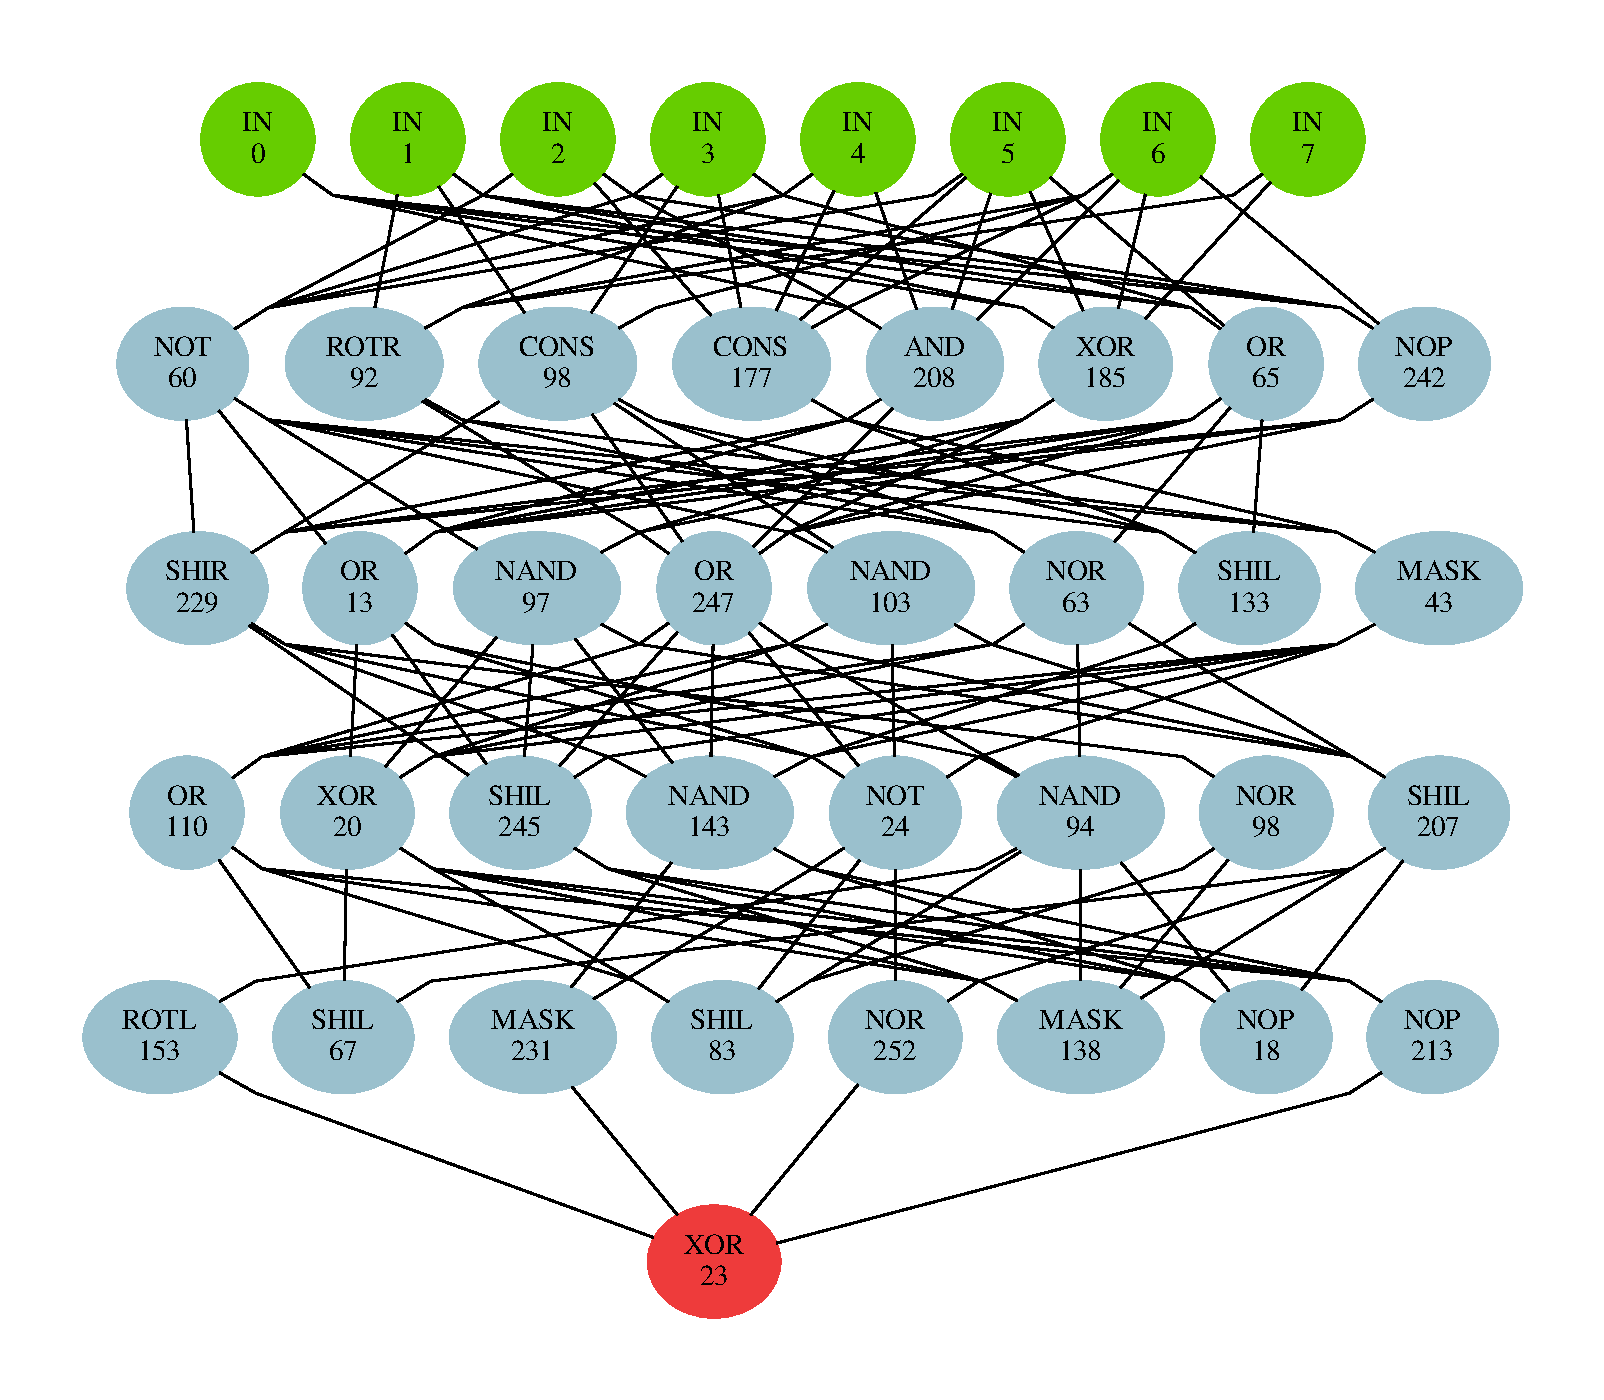
\includegraphics[width=\textwidth]{./graphics/ils/circuit}
  \caption{An iterated local search circuit before pruning.}
  \label{fig:ils-circuit-unpruned}
\end{subfigure}% % this comment has to be here
\begin{subfigure}{.65\textwidth}
  \centering
  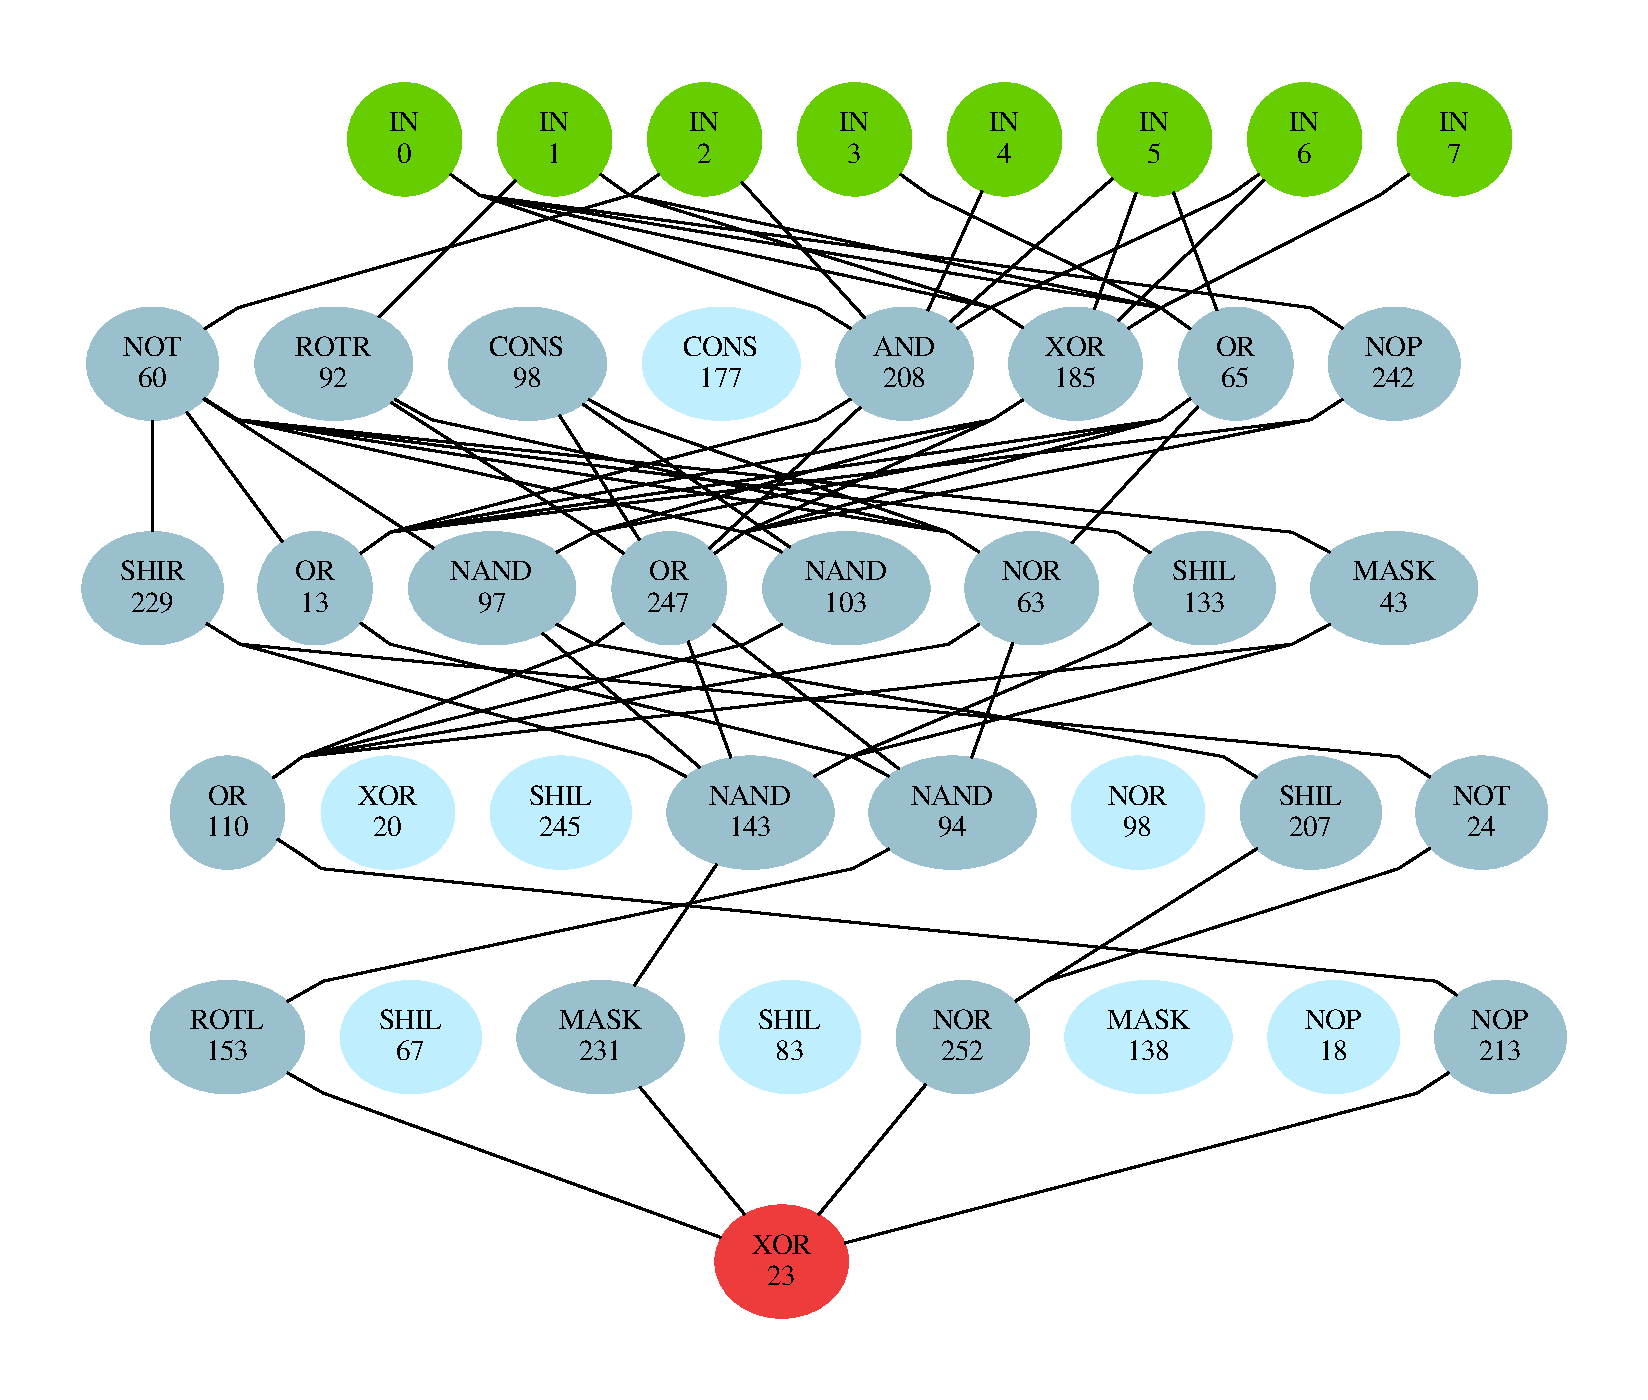
\includegraphics[width=\textwidth]{./graphics/ils/pruned}
  \caption{An iterated local search circuit after pruning.}
  \label{fig:ils-circuit-pruned}
\end{subfigure}

\begin{subfigure}{.65\textwidth}
  \centering
  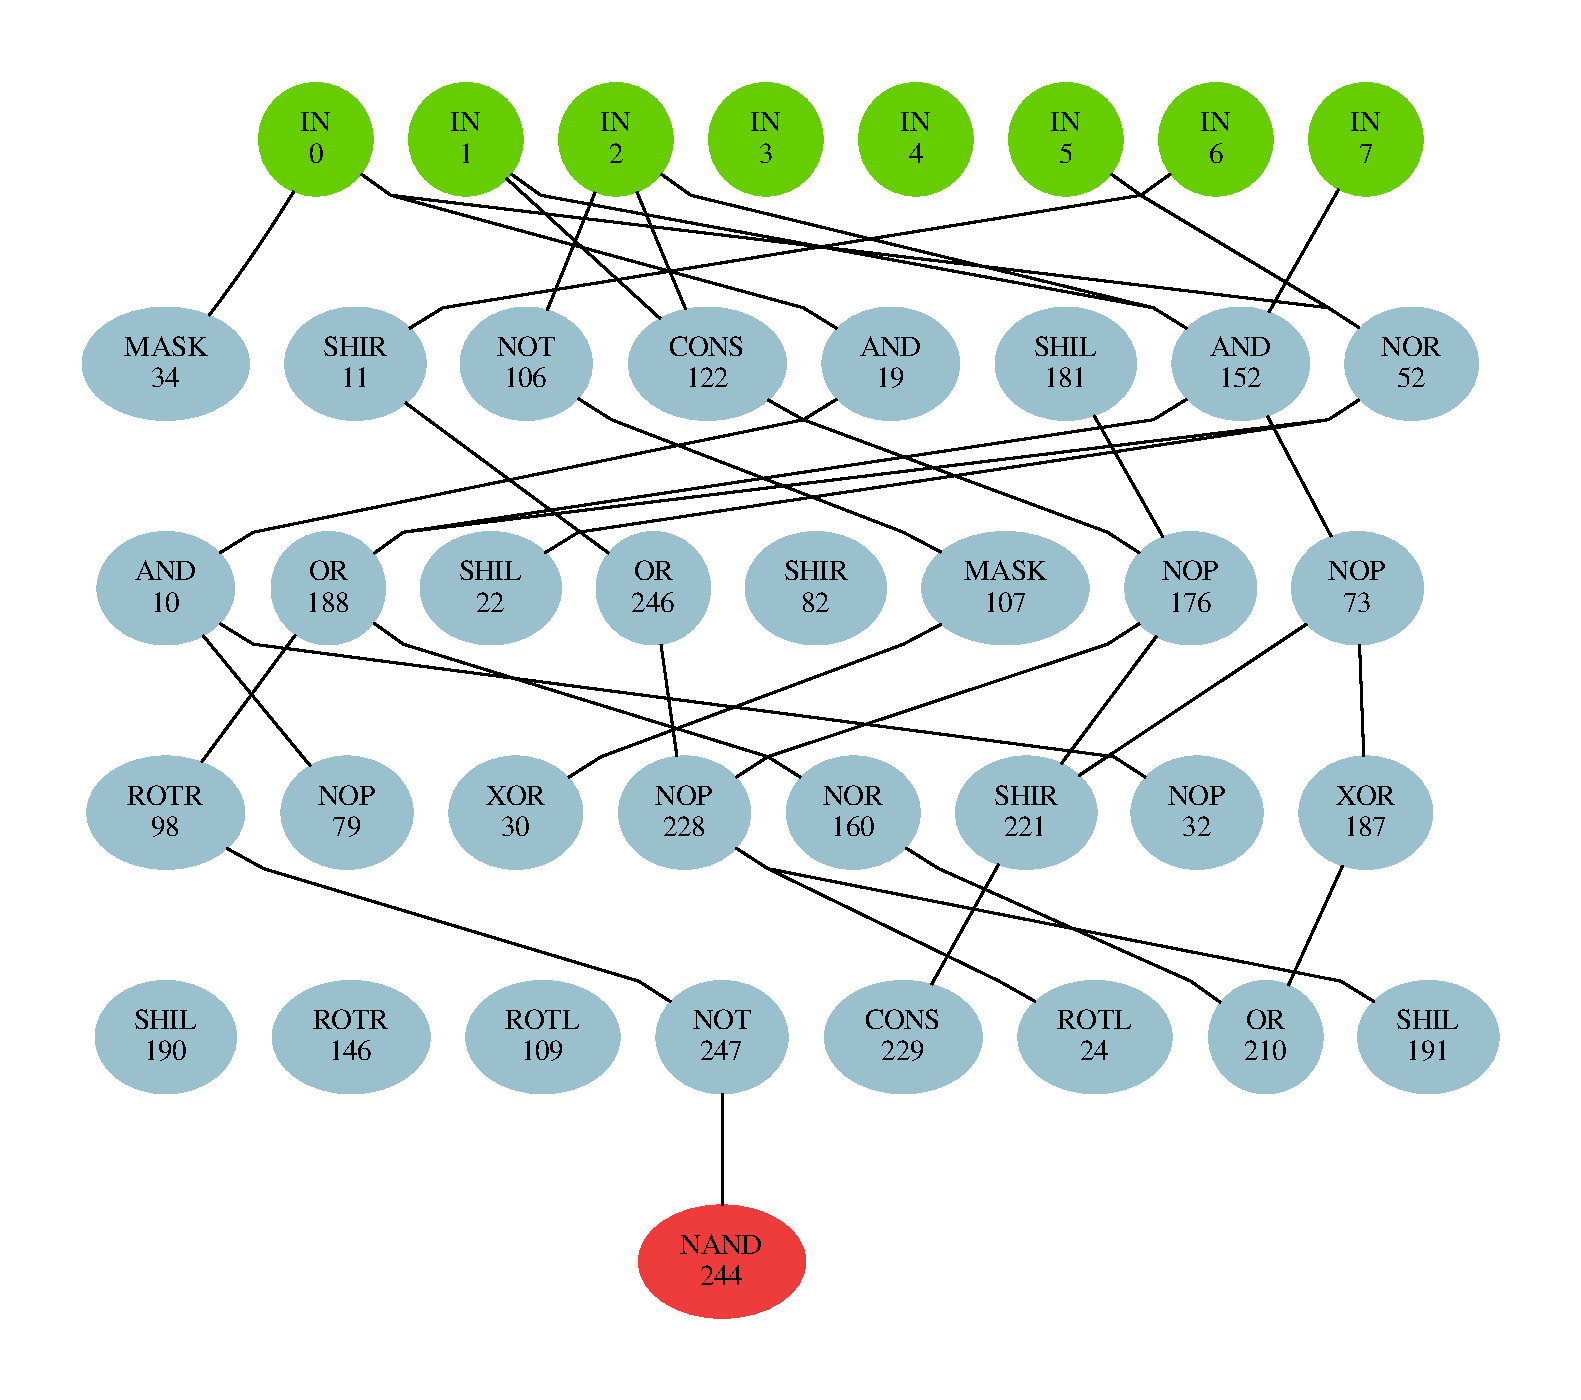
\includegraphics[width=\textwidth]{./graphics/gls/circuit}
  \caption{A guided local search circuit before pruning.}
  \label{fig:gls-circuit-unpruned}
\end{subfigure}% % this comment has to be here
\begin{subfigure}{.65\textwidth}
  \centering
  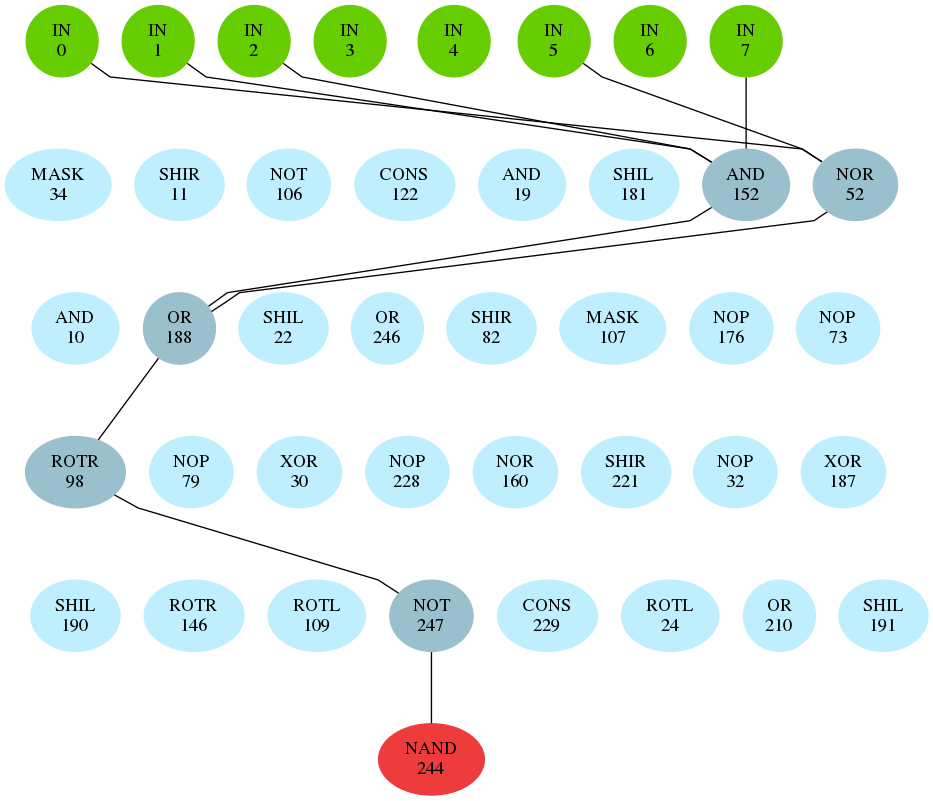
\includegraphics[width=\textwidth]{./graphics/gls/pruned}
  \caption{A guided local search circuit after pruning.}
  \label{fig:gls-circuit-pruned}
\end{subfigure}
\end{changemargin}
\caption{The top two circuits were produced by iterated local search, while bottom two by guided local search. The tested data for all the cases were two-round AES. While the both unpruned and pruned iterated local search circuits are quite dense, even the unpruned guided local search circuit is sparse. However, if the tested data seems random, the guided local search circuit would be even denser than \cref{fig:ils-circuit-unpruned}.}
\label{fig:ils-gls-circuits}
\end{figure}

\subsection{Variable neighbourhood search}
\label{subsec:res-circ-anal-vns}

As in \cref{subsec:res-circ-anal-gls}, we inspected the density of the output circuit. Again, the circuits were on average sparser than circuits from iterated local search. However, they were significantly denser than circuits from guided local search runs. The observation may also support the hypothesis that limiting the neighbourhood is too strict, and disallows valuable changes in the learning process.

%Martin checked


\section{Artificial neural networks}
\label{sec:res-ann}

We analysed artificial neural networks on the same dataset. The algorithm takes two binary files as an input -- the tested data and the referential random data. The first step is encoding the data to a \texttt{NumPy} array of \texttt{floats}. Then we form two mutually exclusive datasets -- the learning and the testing dataset. Both contain randomly chosen test vectors from either of the input files, together with the label of the data source.

We implemented the neural network in the Python library Keras~\cite{chollet2015keras}, which is a high-level API for TensorFlow~\cite{abadi2016tensorflow}. Keras allows simple prototyping of network layout, while TensorFlow is a highly effective implementation of linear algebra for neural networks capable of computation on CPU and GPU. The implementation is entirely independent of the EACirc, and the code is published on GitHub~\cite{EANet}.

We initially designed the network's layout by intuition, trial and error and available tips for networks layout from the best practices of image processing. We designed a network with five layers layout. The input layer's width depends on test vector length. Usually it is 128 bits, encoded as \texttt{floats}. Then follow three hidden layers with widths eight, four, and two neurones. The output layer consists of a single neurone.

We analysed the performance of such prototype network and selected a benchmarking function for the comparison of the influence of network's parameters. We tested multiple layouts. The layout of the prototype network can be noted by a number of neurones in the hidden and output layers -- 8-4-2-1. We experimented with following layouts: 1, 16-1, 8-4-2-1, 8-8-8-1, and 16-8-4-2-1. The second tested parameter of the network was the number of test vectors evaluated in a single iteration. Our preliminary results on the prototype network showed that smaller batches lead to better results. We analyse two properties of the execution: what was the final \textit{acceptance rate} of the network and how fast did the network learned the first statistically significant distinguisher. The \textit{acceptance rate} is equal to the ratio of $\frac{\#_{\textnormal{correct guesses}}}{\#_{\textnormal{total guesses}}}$.

\begin{table}[b]
\centering
\begin{tabular}{l|l l l l l l l}
Layout\textbackslash{}batch size & 10 & 25 & 50 & 100 & 250 & 500 & 1000\\ \hline
1          & 0.985 & 0.967 & 0.957 & 0.934 & 0.937 & 0.641 & 0.716 \\
16-1       & 0.992 & 0.970 & 0.960 & 0.935 & 0.938 & 0.665 & 0.719 \\
8-4-2-1    & 0.525 & 0.663 & 0.510 & 0.581 & 0.605 & 0.505 & 0.500 \\
8-8-8-1    & 0.515 & 0.632 & 0.736 & 0.617 & 0.652 & 0.549 & 0.562 \\
16-8-4-2-1 & 0.516 & 0.500 & 0.503 & 0.507 & 0.504 & 0.506 & 0.518  
\end{tabular}
\caption{The final \textit{acceptance rate} of the artificial neural network on two-round Salsa20 for different parametrizations. Rows describe the used layout and columns represents the size of the batch.}
\label{table:res-ann-acc}
\end{table}

\begin{table}[t]
\centering
\begin{tabular}{l|l l l l l l l}
Layout\textbackslash{}batch size & 10 & 25 & 50 & 100 & 250 & 500 & 1000\\ \hline
1          & 1 & 1 & 0 & 1 & 2 & 10 & 9 \\
16-1       & 2 & 2 & 1 & 6 & 4 & 31 & 20 \\
8-4-2-1    & -- & 53 & -- & -- & 96 & -- & -- \\ 
8-8-8-1    & -- & 76 & 47 & 76 & 63 & -- & -- \\
16-8-4-2-1 & -- & -- & -- & -- & -- & -- & --  

\end{tabular}
\caption{The parametrizations analysis of the neural network on two-round Salsa20. The cell contains the iteration number when the \textit{acceptance rate} overcome 0.6. Rows describe the used layout and columns represents the size of the batch.}
\label{table:res-ann-speed}
\end{table}

An interpretation of the observations from the \cref{table:res-ann-acc,table:res-ann-speed} are the following.

\begin{itemize}
    \item An increasing batch size decreases the learning speed, as can be seen in \cref{table:res-ann-speed}. Our reasoning for this observation is that more testing vectors per one iteration overload the network with too much information. An ideal batch size can be from 10 up to 50 test vectors.
    \item Complex networks learn slower than simple networks. Sometimes the complex networks are not able to learn from the data at all. Nevertheless, the network of a single neurone performs always the best over all the examined batch sizes. The single neurone can still observe if the test vector contains more ones than zeroes as well as simple patterns.
    \item The learning capabilities of the neural networks in our implementation are limited. Based on these observations, we cannot expect neural network is performing better than EACirc.
\end{itemize}

We evaluated one of the best working parametrisation (single neurone and batch size 25) of the neural network on the well-known cryptographic functions dataset. The results are in the \cref{table:res-usable-ann} where rows and cells are same as in the previous results in the \cref{table:res-usable-ils} and in the cell is a final acceptance rate of the run. The \textit{acceptance rate} is equal to the ratio of $\frac{\#_{\textnormal{correct guesses}}}{\#_{\textnormal{total guesses}}}$. It measures the quality of the ANN, similarly as a fitness function was the metaheuristics' metric. The colours have the same meaning as before, the \textit{critical value} used for rejection of randomness was set to 0.554, as such results have probability lower than 1\,\%.

\begin{table}[t]
\centering
\begin{tabular}{l|l l l l}
Function\textbackslash{}rounds & -1 & 0 & 1 & 2\\ \hline
rnd\_rnd$_{\textnormal{no rounds}}$& -- & \fn{}0.503 & --         & --         \\\\
AES$_{3}$        & \fd{}1.0   & \fn{}0.499 & \fn{}0.504 & \fn{}0.503 \\
BLAKE$_{1}$      & \fd{}1.0   & \fn{}0.490 & \fn{}0.500 & \fn{}0.502 \\
Grain$_{2}$      & \fd{}1.0   & \fd{}1.0   & \fn{}0.496 & \fn{}0.494 \\
Gr\o stl$_{2}$   & \fn{}0.495 & \fn{}0.495 & \fn{}0.495 & \fn{}0.496 \\
HC-128$_{\textnormal{no rounds}}$& --    & \fn{}0.492 & -- & --      \\
JH$_{6}$         & \fd{}1.0   & \fd{}1.0   & \fn{}0.494 & \fn{}0.497 \\
Keccak$_{3}$     & \fd{}0.992 & \fn{}0.496 & \fn{}0.502 & \fn{}0.495 \\
MD6$_{8}$        & \fd{}0.706 & \fn{}0.490 & \fn{}0.500 & \fn{}0.501 \\
Rabbit$_{0}$     &      --    & \fn{}0.456 & \fn{}0.504 & \fn{}0.512 \\
RC4$_{\textnormal{no rounds}}$& --         & \fn{}0.502 & --         & --         \\
Salsa20$_{2}$    & \fd{}0.996 & \fd{}0.985 & \fn{}0.500 & \fn{}0.502 \\
SINGLE-DES$_{4}$ & \fn{}0.536 & \fn{}0.501 & \fn{}0.500 & \fn{}0.498 \\
Skein$_{3}$      & \fd{}1.0   & \fd{}0.632 & \fn{}0.480 & \fn{}0.464 \\
SOSEMANUK$_{4}$  & \fd{}1.0   & \fd{}1.0   & \fn{}0.476 & \fn{}0.456 \\
TEA$_{4}$        & \fn{}0.512 & \fn{}0.500 & \fn{}0.495 & \fn{}0.496 \\
TRIPLE-DES$_{2}$ & \fd{}0.999 & \fd{}0.596 & \fn{}0.506 & \fn{}0.501
\end{tabular}
\caption{The best-obtained results of ANN on well-known cryptographic functions dataset. The values are corresponding to \textit{acceptance rate}, where value $0.5$ is expected for runs that cannot reject the randomness hypothesis of the tested data. The dash represents a scenario that was not tested.}
\label{table:res-usable-ann}
\end{table}

We also experimented with convoluted neural networks (CNN). The convoluted neural network works excellent for image and signal processing, as the convoluted layer detects local patterns. However, cryptographic functions should meet the strict avalanche criterion suppressing any data locality. The CNN serves as a specific test for locality-specific patterns. If the reduced cryptographic function meets the strict avalanche criterion, the CNN should perform worse, as the first layer of CNN has lower capabilities than a fully connected layer of ANN.

Overall, the CNN performed worse than ANN. The problems were slower learning than ANN, and sometimes the distinguisher was not found even during more epochs.

%\subsection{Analysis of the neural network learning progress}
%\label{subsec:res-ann-learn}

%An analysis of ANN learning can be evaluated by following two variables.

%\begin{description}
    %\item[Acceptance rate] is equal to ratio of $\frac{\#_{\textnormal{correct quesses}}}{\#_{\textnormal{total quesses}}}$. So it measures the quality of the ANN, similarly as fitness function was the metaheuristics' metric.
    %\item[Crossentropy loss] describes how big changes can the network do for learning itself (similar to the temperature of simulated annealing). %TODO cite
%\end{description}

%Those values are shown for AES in 1 to 3 rounds with both ANN and CNN for comparison in \cref{fig:ann-learning}.

%\begin{figure}[H]
%\begin{changemargin}{-3cm}{-3cm}
%\centering
%\begin{subfigure}{.6\textwidth}
  %\centering
  %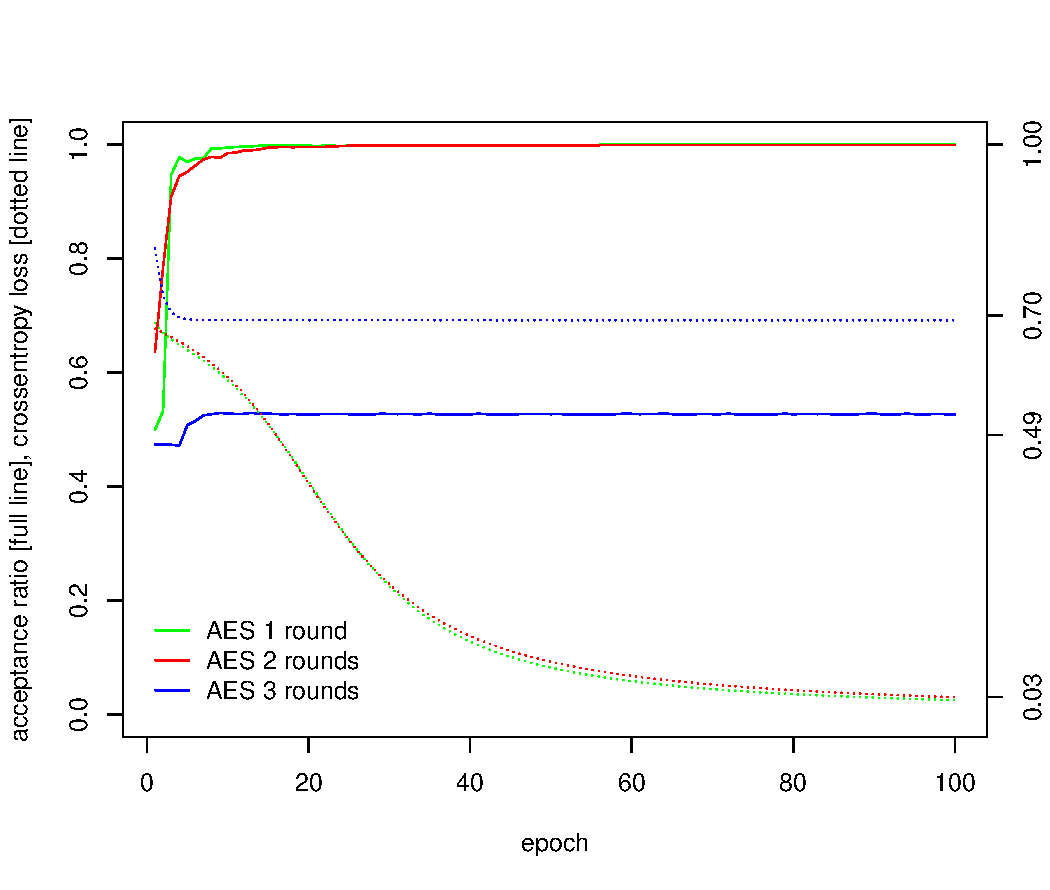
\includegraphics[width=.98\textwidth]{./graphics/ann/ann}
  %\label{fig:ann-learning-ann}
%\end{subfigure}% % this comment has to be here
%\begin{subfigure}{.6\textwidth}
  %\centering
  %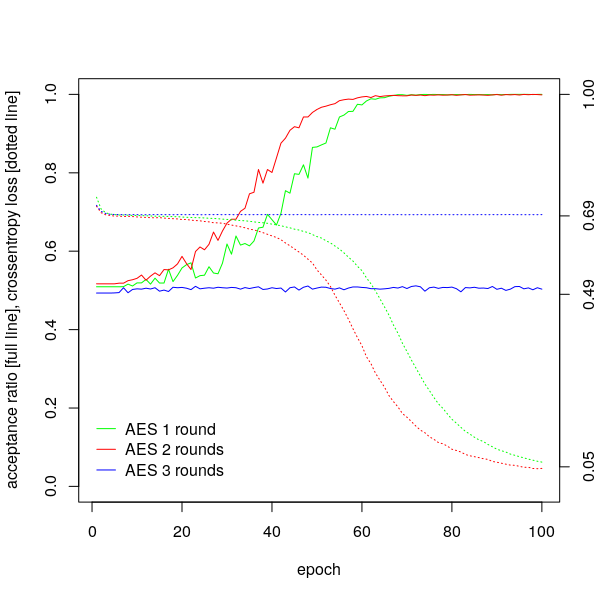
\includegraphics[width=.98\textwidth]{./graphics/ann/cnn}
  %\label{fig:ann-learning-cnn}
%\end{subfigure}
%\end{changemargin}
%\caption{Learning process of ANN (left) and CNN (right) on AES reduced to one to three rounds.}
%\label{fig:ann-learning}
%\end{figure}


\section{Inter-approach comparison}
\label{sec:res-comp}

The interesting details about single-solution metaheuristics are summarised in \cref{table:ss-comparison}. The artificial neural network models are omitted in the table. They are not able to detect non-randomness of functions reduced to the given number of rounds, except eight rounds MD6. The summary is presented below.

\begin{table}
\centering
\begin{tabular}{l|l l l l}
Function\_rounds\textbackslash{}Metaheuristic   & \rot[90]{Iterative local search} & \rot[90]{Simulated annealing} & \rot[90]{Guided local search} & \rot[90]{Variable neighbourhood search} \\ \hline
AES$_3$     & \fd{}0.160         & \fd{}\textbf{0.305}    & \fd{}0.164             & \fd{}0.182         \\
BLAKE$_1$   & \fd{}0.110         & \fd{}0.051             & \fd{}\textbf{0.260}    & \fd{}0.157         \\
MD6$_8$     & \fd{}0.774         & \fd{}0.419             & \fd{}\textbf{0.995}    & \fd{}0.992         \\
DES$_5$     & \fd{}0.204         & \fd{}0.093             & \fd{}\textbf{0.496}    & \fd{}0.441         \\
TEA$_4$     & \fd{}0.444         & \fd{}0.244             & \fd{}0.729             & \fd{}\textbf{0.877}
\end{tabular}
\caption{The \textit{rejection rate} for selected cryptographic functions of EACirc utilising different single-solution metaheuristics.}
\label{table:ss-comparison}
\end{table}


\begin{itemize}
    \item Guided local search is always more successful than the baseline iterated local search, and it is almost always the best among the tested methods. The single better result of simulated annealing does not mean it is better than guided local search, due to the higher \textit{empirical critical value} caused by the \textit{connection bug}. The same holds for four-round TEA and variable neighbourhood search, as it has a longer computation time.
    \item The ANN can detect bit-level non-randomness, while EACirc cannot. The bit-oriented evaluation is expected to to be crucial for the cryptanalysis. However, this did not lead to the creation of ANN distinguisher for any function, that would EACirc not be able to distinguish.
    \item The runtime of the simulated annealing and the guided local search is the same as the runtime of the iterated local search. The variable neighbourhood search can take up to five times longer. The data consumption of all metaheuristics in EACirc is the same, as described in \cref{fig:dataUsage}.
    
    In comparison, the neural networks need significantly less data (as was shown in \cref{fig:ann-dataUsage}). One run of ANN takes about ten times less time than one EACirc run. However, due to varying capabilities, these numbers are not comparable. EACirc can also find distinguishers for the two-round AES within less than ten epochs, even though we set 300 \textit{epochs} as the default. Interesting comparison of the efficiency of EACirc implementation is that \texttt{C++} EACirc consumes twelve times more data per second of computation than ANN implemented in \texttt{Python}.
    
    Still, the ANN is the only method, which can be used to classify a single test vector (16 bytes). The framework provides both its classification guess and the estimation of its certainty in the guess. No other method provides such application. EACirc is not able to classify a single vector in the current setting due to the statistical evaluation described in \cref{chap:eacirc}. Nevertheless, EACirc can be set to evaluate a single test vector. Such setting was used by Ukrop in~\cite{ukropBcThesis}.
\end{itemize}

\chapter{Related work}
\label{chap:relatwork}

We presented our tools for randomness assessment, yet this area is broad, and many researchers developed their own tools. Most commonly, the tools are not adaptive to the data. Instead, they test the data for a set of statistical properties. These statistical tests are grouped to statistical test batteries. There are multiple batteries, we present the followings.

%Assesment of randomness is necessary in other fields than just cryptography. Physicists use randomness assesment for .... Overal, all research areas need to evaluate their data by statisticaal tests. Therefore, statistical testing is well studied field with multiple standard tools. There are multiple statistical batteries. 

\begin{description}
    \item[Donald Knuth] explains statistical testing in the second edition of The Art of Computer Programming~\cite{knuth1969vol}. He suggested several PRNGs, and for analysis, he designed some statistical tests. The high quality of this source discouraged other researchers from work in this area until George Marsaglia came with the Diehard battery. \todo{cite discouraged} %zeroth
    \item[Diehard] was developed at Florida State University by George Marsaglia in 1995~\cite{marsaglia1996diehard}. It was published on CD together with three so-called true random data sources and multiple PRNGs. %first
    \item[Crypt-X suite] was a test battery for analysis of cryptoprimitives used in the late nineties~\cite{cryptxs}. NIST STS fully surpassed it. % second
    \item[NIST STS] is the golden standard of statistical testing in cryptography~\cite{rukhin2001statistical}. NIST standardised part of the battery as one step for certification FIPS FIPS 140-2. It was also used as one criterion of evaluation of AES candidates, evaluated by Murphy in~\cite{murphy2000power}. For example, Murphy found that the AES candidate HPC failed in NIST STS, which detected possible weaknesses of the algorithm.

    NIST STS was developed in the late nineties, and the last revision was released in 2010~\cite{rukhin2001statistical}. The 2010 update removed biased test \textit{Lempel-Ziv Complexity of Sequences}. Further analysis of the bias in the $p$-values produced by NIST STS shows more dependent tests, which leads to a production of biased results. Overall NIST STS is accepted as a "golden" standard, so newer batteries extend it (at least the FIPS 140 subset of NIST STS battery) and relates to it. % third
    \item[Dieharder] was developed by Robert G. Brown at the Duke University in 2004~\cite{brown2013dieharder}. It reimplements all tests of Diehard battery, and extends it by many additional tests. Dieharder also contains three of fifteen test of NIST STS battery. However, it suffers similar bias flaws as NIST STS, as detected \todo{Lubo in}. % fourth
    \item[TestU01] is state of the art in statistical testing. It is a library, continuously developed by Université de Montréal since 2007~\cite{l2007testu01}. The design of the test is innovative in comparison to previous batteries. It uses fewer tests, whose are parametrised to form more sub-tests. This approach outperforms all other statistical batteries, as will be shown in our results in \cref{table:res-batteries}. The TestU01 also implements multiple PRNG from different categories, observing the same results, which proves the non-randomness. % fifth
    \item[PractRand] is another competitor to TestU01~\cite{dotypractically}. The author claims PracRand suits better for testing a large amount of data in comparison to other batteries. However, we have not testified this claim.
    \item[RaBiGeTe] is user friendly battery for Windows users~\cite{rabigete}. It implements some of the NIST STS's tests and some of Donald Knuth's tests.
\end{description}

There are also others statistical batteries: CryptoStat~\cite{kaminsky2013cryptostat}, YAARX~\cite{biryukov2014automatic}, ENT~\cite{walker2008ent}, SPRNG~\cite{mascagni2000algorithm}, gjrand~\cite{gjrand} and BSI test suite~\cite{schindler2002evaluation}. \todo{Petr: proc vsechny necitujes? Proc o nich neni neco uvedeno? }

% randomness is analysed in more research areas
%   statistical batteries
%       find use-cases
%       papers on stat bat in crypto (paper of NIST STS for AES competition)
% more papers on randomness analysis (in crypto) // take inspiration in TEA paper

\section{Statistical batteries}
\label{sec:relatwork-stat}

% what they are
% methodics

We evaluated the dataset of well-known functions with NIST STS (faster implementation by Sýs et al. was used~\cite{sys2016algorithm}), Dieharder and TestU01 battery. Those batteries were automated in the project Randomness testing toolkit (RTT)~\cite{rttgit} as part of the master thesis of Lubomír Obrátil~\cite{obratilMgrThesis}. RTT is online service, which allows the user to upload binary data and it executes the batteries on them. It automatically detects the best possible setting of the batteries, as they are parametrised mainly by the size of the binary file. After the execution, RTT postprocess the results and outputs human readable interpretation of them. Same as the visualisation in this thesis, it uses colours to simplify the interpretation, where red stands for rejected test and green for passed test.

Such interpretation is straightforward. However, we show it may be incorrect in a very specific situation due to statistical properties of the batteries. To prove that, we need to explain the interpretation in a statistical manner.

A single test assesses the data against the null hypothesis that the data are random. The test may reject the hypothesis and therefore state the data seems nonrandom, or it may accept the hypothesis, where it means the test cannot find enough evidence for nonrandomness of the data. However, the test may fail with an error of two types.

\begin{description}
    \item[Type I error] describes the likelihood of acceptance null hypothesis when it is false (false positive). The test incorrectly states that the data are not random. This error occurs with the probability specified by significance level $\alpha$ for random data.
    \item[Type II error] describes the likelihood of rejection null hypothesis when it is true (false negative). The test did not spot nonrandomness of the data. The probability of type II error is also dependent on $\alpha$, and its calculation is denoted $\beta$.
\end{description}

The batteries consist of a set of tests, that are parametrised up to hundreds of sub-tests. If the significance level $\alpha$ is, for example, $1\,\%$, then the probability that all 100 tests will correctly pass is $0.99^{100}=36.6\,\%$ (suppose the tests are independent, which however do not hold for sub-tests). Therefore, we have to expect type I errors. The probability of type I error further increases if the tests are dependent. Sýs et al.~\cite{sys2015interpretation} showed that some of the NIST STS tests are dependent and they proposed the interpretation of the battery based on calculated proportion of failed tests. Same authors plan to revise also Dieharder battery, which contains similar ambiguity in interpretation. Part of these results are going to be published in thesis of Lubomír Obrátil~\cite{obratilMgrThesis}. RTT uses this approach for the interpretation.

\subsection{Statistical batteries results}
\label{subsec:relatwork-stat-res}

The comparison of multiple batteries can be seen in \cref{table:res-batteries}. The visualisation required changes of the table. The rows of the table represent cryptographic functions reduced to the given number of rounds. These functions with rounds may repeat, if different statistical testing tools were able to detect non-randomness of the function reduced to a different number of rounds. The column represents single statistical battery or EACirc tool with guided local search metaheuristic. The contains the number of failed sub-tests of total sub-tests from the table header or EACirc's \textit{rejection rate}. Or interpretation of the randomness is signalised by the highlight. The red colour signalises the tool rejected randomness hypothesis, the cell is green othervise.

\begin{table}[H]
\centering

\scalebox{0.95}{
\begin{tabular}{@{}l|rrrrrrrrrr@{}}
\textbf{\large Algorithm} & 
\multicolumn{1}{R{3.2cm}}{\textbf{NIST STS} \\ \footnotesize (x/15)} &
\multicolumn{1}{R{3.2cm}}{\textbf{Dieharder} \\ \footnotesize (x/27)} &
\multicolumn{1}{R{3.2cm}}{\textbf{Small Crush} \\ \footnotesize (x/10)} &
\multicolumn{1}{R{3.2cm}}{\textbf{Crush} \\ \footnotesize (x/32)} &
\multicolumn{1}{R{3.2cm}}{\textbf{Rabbit} \\ \footnotesize (x/16)} &
\multicolumn{1}{R{3.2cm}}{\textbf{Alphabit} \\ \footnotesize (x/4)} &
\multicolumn{1}{R{3.2cm}}{\textbf{Block Alphabit} \\ \footnotesize (x/4)} &
\multicolumn{1}{R{3.2cm}}{\textbf{EACirc} \\ \footnotesize (\textit{rejection rate})} \\ \hline
AES$_{3}$                        &  8    \fd & 15 \fd &  5   \fd & 20    \fd &  5 \fd & 2 \fd & 4 \fd & 0.164 \fd \\ \hline
BLAKE$_{1}$                      & 11    \fd & 11 \fd &  5   \fd & 18    \fd &  5 \fd & 2 \fd & 3 \fd & 0.260 \fd \\ \hline
Grain$_{2}^{\ast}$               & 14    \fd & 27 \fd &  9/9 \fd & 31/31 \fd & 15 \fd & 4 \fd & 4 \fd & 1.000 \fd \\
Grain$_{6}^{\ast}$               &  1    \fn &  0 \fn &  0   \fn &  3    \fn &  1 \fn & 0 \fn & 0 \fn & 0.017 \fn \\ \hline
Gr\o{}stl$_{2}$                  & 12    \fd & 23 \fd &  9 \fd   & 27    \fd &  9 \fd & 3 \fd & 3 \fd & 1.000 \fd \\ \hline
JH$_{6}$                         & 12/13 \fd & 27 \fd & 10 \fd   & 30/31 \fd & 15 \fd & 4 \fd & 4 \fd & 1.000 \fd \\ \hline
Keccak$_{2}$                     & 14    \fd & 27 \fd & 10 \fd   & 31    \fd & 15 \fd & 4 \fd & 4 \fd & 1.000 \fd \\
Keccak$_{3}$                     &  0    \fn &  1 \fn &  1 \fn   & 11    \fd &  4 \fd & 0 \fn & 3 \fd & 0.017 \fn \\ \hline
MD6$_{8}^{\ast}$                 &  9    \fd & 19 \fd &  5 \fd   & 16    \fd &  8 \fd & 2 \fd & 3 \fd & 0.995 \fd \\
MD6$_{10}^{\ast}$                &  0    \fn &  0 \fn &  0 \fn   &  2    \fn &  3 \fd & 0 \fn & 0 \fn & 0.016 \fn \\ \hline
Rabbit$_{0}^{\ast}$              &  1    \fn &  1 \fn &  0 \fn   &  4    \fd &  3 \fd & 1 \fn & 1 \fn & 0.017 \fn \\
Rabbit$_{4}^{\ast}$              &  0    \fn &  0 \fn &  0 \fn   &  3    \fn &  3 \fd & 1 \fn & 1 \fn & 0.009 \fn \\ \hline
Salsa20$_{2}$                    & 12    \fd & 26 \fd &  8 \fd   & 28    \fd & 11 \fd & 3 \fd & 3 \fd & 1.000 \fd \\ \hline
Single DES$_{4}$                 &  7    \fd & 22 \fd &  7 \fd   & 26    \fd & 11 \fd & 4 \fd & 4 \fd & 0.496 \fd \\
Single DES$_{5}$                 &  1    \fn &  6 \fd &  1 \fn   & 18    \fd &  5 \fd & 2 \fd & 3 \fd & 0.011 \fn \\ \hline
Skein$_{3}$                      & 12    \fd & 27 \fd & 10 \fd   & 30    \fd & 13 \fd & 3 \fd & 4 \fd & 1.000 \fd \\
Skein$_{4}$                      &  0    \fn &  0 \fn &  0 \fn   & 10    \fd &  4 \fd & 1 \fn & 3 \fd & 0.012 \fn \\ \hline
SOSEMANUK$_{4}$                  & 13/13 \fd & 27 \fd & 10 \fd   & 31/31 \fd & 16 \fd & 4 \fd & 4 \fd & 1.000 \fd \\ \hline
TEA$_{4}$                        &  8    \fd & 19 \fd &  6 \fd   & 15    \fd &  4 \fd & 2 \fd & 3 \fd & 0.729 \fd \\
TEA$_{5}$                        &  0    \fn &  3 \fn &  2 \fn   &  4    \fd &  1 \fn & 0 \fn & 3 \fd & 0.015 \fn \\ \hline
Triple DES$_{2}$                 & 12    \fd & 26 \fd &  9 \fd   & 31    \fd & 15 \fd & 3 \fd & 4 \fd & 1.000 \fd \\
Triple DES$_{3}$                 &  1    \fn &  4 \fd &  1 \fn   &  4    \fd &  0 \fn & 1 \fn & 1 \fn & 0.012 \fn \\ \hline
RC4$_{\textnormal{no rounds}}^{\ast}$ &  0 \fn &  0 \fn &  0 \fn &  3    \fn &  0 \fn & 0 \fn & 0 \fn & 0.008 \fn \\

\end{tabular}
}

\caption{Application of statistical batteries and EACirc on data from round-reduced well-known cryptographic functions. 
The the values in the table are described in \cref{subsec:relatwork-stat-res}.
The results were computed by Randomness Testing Toolkit. Complete results with detailed information about which tests are passing can be found on \href{http://rtt.ics.muni.cz/ViewResults/?created_from=2017-04-24+12\%3A00\%3A00&created_to=2017-04-29+00\%3A00\%3A00}{RTT page (as results from 2017-04-24 to 2017-04-28)}.}
\label{table:res-batteries}
\end{table}

From those results, we have multiple observations.

\begin{itemize}
    \item EACirc performs similarly to NIST STS, Dieharder and TestU01 Small Crush.
    \item TestU01 Crush outperforms all other batteries, which is traded-of by its computation time and the amount of analysed data.
    \item High amount of failed test indicates the data are biased in multiple characteristics. Such data are usually rejected by all batteries. However, when only a single battery detects nonrandomness, it is TestU01.
    \item \textbf{TestU01 was able to detect deviances in full Rabbit cipher.} After analysis of this result, we found that there was a report \textit{On a bias of Rabbit}~\cite{aumasson2007bias} during the eSTREAM competition, which discovered the same property. Even though this bias was found, Rabbit cipher was selected as software profile finalist, stating that the bias does not allow any feasible attack due to complexity.
    \item Similarly observation is the bias of a hardware profile eSTREAM finalist Grain. TestU01 Crush can detect bias up to six rounds Grain, which is almost one-half of the full function (13 rounds). The known \textit{dynamic cube attack} on the same version of Grain~\cite{dinur2011breaking} do not explain the bias observed by us. Our round reduction is based on a limitation of the shuffle of the non-linear feedback shift registers, which may require more than six rounds to shuffle the data enough. The full Grain cipher has 13 rounds, which still provides some security margin.
    \item The interpretation based on the probability of fail of $n$ sub-tests would not detect the nonrandomness property of Grain reduced to five rounds. The rejection approach is strict (so it has hight probability of type II error), however manual observation that the failed sub-tests are the same as failed sub-tests of four and six rounds Grain provide necessary trust to our interpretation that the data are biased. In addition, such results were examined via retesting on different data from the same setting.
    \item Note: MD6 reduced to 10 rounds is nonrandom based on TestU01 Crush and Rabbit. The results in the table were omitted due to consistency, as the interpretation method leaves them as passed test. However, the probability of those extreme results is below 1\,\%. The same behaviour was detected for RC4 by TestU01 Crush.
    \item Rejection of randomness by the battery do not have to be taken as black-box (as we present here), but we can analyse, which test failed. However, depending on the test, it may be more difficult than analysis of the output circuit from EACirc.

    EACirc may also provide concrete proof of the data dependency. If there is a dependency between specifics bytes, it would always be present in the circuit for strong distinguishers. The statistical battery would some test, probably the \textit{dependency test}. However, they would not state, what is the dependence in the data.
    \item Another advantage of EACirc is the simplicity of already learned distinguisher. Using learned distinguisher needs much less data, only low kilobytes and it may even state the guess for a single test vector. The test of statistical battery always requires fixed amount of data.
\end{itemize}

\section{Compression algorithms}
\label{sec:relatwork-compress}

One of the definitions of randomness is via Kolmogorov's complexity. Data are random if they cannot be compressed. The data from the cryptographic function can always be compressed, but the computation would require finding the key used for the encryption; therefore such compression is not feasible.

We experimented with this approach, trying capabilities of compression programs. We have analysed following Unix lossless data compression utilities.

\begin{description}
    \item[zip] is compression utility based on Deflate algorithm. It combines LZ77~\cite{ziv1977universal} and Huffman coding algorithms.
    \item[gzip] is GNU version of \textit{zip} utility.
    \item[lzop] is compression utility using LZO algorithm. It aims for faster decompression; however, the compression can be less efficient than \textit{gzip}.
    \item[bzip2] is compression algorithm based on Burrows–Wheeler transformation~\cite{burrows1994block} of the reoccurring sequences to strings of identical letters. Then it applies the move-to-front transformation and Huffman coding. 
    \item[NanoZip] in version 0.09a is the latest version from the year 2011 of an experimental archiver software based on Burrows-Wheeler compression~\cite{nanozip}. Based on multiple data compression benchmarks, NanoZip has the highest compression capabilities. Although we used various parameters, we did not obtain archive, which could be losslessly decompressed. Therefore we omit this algorithm.
\end{description}

All the utilities were executed with highest compression ratio with the slowest speed.

We denote the results in a similar manner as results of the batteries. The rows are labelled by cryptographic functions, columns are compression utilities. The cell is a pair of the round count that we executed the algorithm, and compression ratio, which says how much data we safe. Compression of random data should not safe anything, marked with dash, whatever higher means the data are nonrandom. We tested this evaluation experimentally on random data, and the compressed file was never smaller than the original file. This property was tested for more than ten samples. The dash means that the compression algorithm was unable to detect nonrandomness compress the data from any reduced version of the cryptographic function.

\begin{table}[t]
\centering

\scalebox{0.95}{
\begin{tabular}{@{}l|lllll@{}}
\textbf{\large Algorithm} & 
\multicolumn{1}{R{1.3cm}}{\textbf{bzip2}} &
\multicolumn{1}{R{1.3cm}}{\textbf{gz}} &
\multicolumn{1}{R{1.3cm}}{\textbf{lzop}} &
\multicolumn{1}{R{1.3cm}}{\textbf{zip}} &
\multicolumn{1}{R{1.3cm}}{\textbf{ANN}} \\ \hline
AES$_{2}$                        & 2.  \fd & 15. \fd & 25. \fd & 15. \fd & 1.0   \fd \\ \hline
BLAKE$_{0}$                      & 0.  \fd & 0.  \fd & 1.  \fd & 0.  \fd & 1.0   \fd \\ \hline
Grain$_{2}$                      & 3.  \fd & 11. \fd & 25. \fd & 11. \fd & 1.0   \fd \\ \hline
Gr\o{}stl$_{0}$                  & 0.  \fd & 0.  \fd & 1.  \fd & 0.  \fd & 1.0   \fd \\ \hline
HC-128$_{0}$                     & --  \fd & --  \fd & --  \fd & --  \fd & 0.492 \fd \\ \hline
JH$_{6}$                         & 57. \fd & 59. \fd & 68. \fd & 59. \fd & 1.0   \fd \\ \hline
Keccak$_{1}$                     & 16. \fd & ++. \fd & 36. \fd & ++  \fd & 1.0   \fd \\
Keccak$_{2}$                     & --  \fn & 99. \fn & --  \fn & 99. \fd & 0.992 \fd \\ \hline
MD6$_{6}$                        & ++  \fd & ++  \fd & 59. \fd & ++  \fd & 1.0   \fd \\
MD6$_{7}$                        & 99. \fn & 97. \fn & --  \fn & 97. \fn & 0.706 \fd \\ \hline
Rabbit$_{0}$                     & --  \fn & --  \fn & --  \fn & --  \fd & 0.456 \fd \\ \hline
RC4$_{\textnormal{no rounds}}$   & --  \fn & --  \fn & --  \fn & --  \fn & 0.502 \fn \\ \hline
Salsa20$_{2}$                    & --  \fd & 99. \fd & --  \fd & 99. \fd & 0.985 \fd \\ \hline
Single DES$_{2}$                 & 71. \fd & 79. \fd & 84. \fd & 78. \fd & 0.824 \fd \\ \hline
Skein$_{2}$                      & 93. \fd & 79. \fd & 93. \fd & 80. \fd & ++ \fd \\ \hline
SOSEMANUK$_{4}$                  & 0.  \fd & 0.  \fd & 1.  \fd & 0.  \fd & 1.0   \fd \\ \hline
TEA$_{2}$                        & 97. \fd & ++  \fd & 93. \fd & ++  \fd & 0.932 \fd \\
TEA$_{3}$                        & --  \fn & 99. \fn & --  \fn & 88. \fd & 0.512 \fn \\ \hline
Triple DES$_{2}$                 & 99. \fd & 98. \fd & 99. \fd & 98. \fd & 0.999 \fd \\
Triple DES$_{2}$                 & --  \fd & --  \fd & --  \fd & --  \fd & 0.596 \fd \\

\end{tabular}
}

\caption{Capabilities of compression algorithms on cryptographic data. Cell contain pair of highest number of rounds, to which was the cryptographic function reduced and saved space ratio of the compression.}
\label{table:res-compression}
\end{table}

\begin{table}[t]
\centering{}
\begin{tabular}{l|p{1.8cm} p{1.8cm} p{1.8cm} p{1.8cm}}
Function\textbackslash{}algorithm & 
                bzip2   &   gz      &   lzop    &   zip     \\ \hline
AES         & 2, 2\,\%  & 2, 15\,\% & 2, 25\,\% & 2, 15\,\% \\
BLAKE       & 0, 0\,\%  & 0, 0\,\%  & 0, 1\,\%  & 0, 0\,\%  \\
Grain       & 2, 3\,\%  & 2, 11\,\% & 2, 25\,\% & 2, 11\,\% \\
Grostl      & 0, 0\,\%  & 0, 0\,\%  & 0, 1\,\%  & 0, 0\,\%  \\
HC-128      & --        & --        & --        & --        \\
JH          & 6, 57\,\% & 6, 59\,\% & 6, 68\,\% & 6, 59\,\% \\
Keccak      & 1, 16\,\% & 2, 99\,\% & 1, 36\,\% & 2, 99\,\% \\
MD6         & 7, 99\,\% & 7, 97\,\% & 6, 59\,\% & 7, 97\,\% \\
Rabbit      & --        & --        & --        & --        \\
RC4         & --        & --        & --        & --        \\
Salsa20     & --        & 2, 99\,\% & --        & 2, 99\,\% \\
SINGLE-DES  & 2, 71\,\% & 2, 79\,\% & 2, 84\,\% & 2, 78\,\% \\
Skein       & 2, 93\,\% & 2, 79\,\% & 2, 93\,\% & 2, 80\,\% \\
SOSEMANUK   & 4, 0\,\%  & 4, 0\,\%  & 4, 1\,\%  & 4, 0\,\%  \\
TEA         & 2, 97\,\% & 3, 99\,\% & 2, 93\,\% & 3, 99\,\% \\
TRIPLE-DES  & 2, 99\,\% & 2, 98\,\% & 2, 99\,\% & 2, 98\,\% 

\end{tabular}
\caption{Capabilities of compression algorithms on cryptographic data. Cell contain pair of highest number of rounds, to which was the cryptographic function reduced and saved space ratio of the compression.}
\label{table:res-compression}
\end{table}

Observations from the results are following.

\begin{itemize}
    \item The efficiency of newer \textit{bzip2} on cryptographic data is not higher than efficiency of \textit{gzip} and \textit{zip}.
    \item The fact that we have to reduce functions to very few rounds is probably caused by character (byte-level) specialisation of the compression algorithms. The cryptographic data may contain more bit-level dependencies.
    \item Still the compression algorithms state similarly to results of neural networks. From these results, we can assume that neural networks detected only the disproportion of zeroes and ones or simple byte-level patterns.
\end{itemize}


\section{Metaheuristcs for randomness testing}
\label{sec:relatwork-paper}

Besides statistical batteries, numerous other works did the cryptanalysis based on testing some of the statistical properties. We have encountered several works using genetics for statistical analysis of cryptoprimitives. Most of them analysed Tiny Encryption Algorithm (TEA), which is a simple block cipher designed by D. Wheeler and R. Needham in 1995~\cite{TEA}. It was used as a benchmark due to its simplicity and well-known vulnerabilities~\cite{TEAAttack}. The application of genetics programming started in 2002 by J. Hernández et al.~\cite{twoRoundsTea}, whose found statistical deviance in two rounds TEA. Further improvements from the team were presented in 2004 finding the non-randomness in three and four rounds TEA as well~\cite{fourRoundsTea}. So far the best results using genetic programming were found by W. Hu~\cite{fiveRoundsTea}, who detected non-random properties for five rounds TEA. We compared EACirc with these results in~\cite{2016-infocommunications-kubicek}.

The Genetic programming was also used for analysis of four rounds DES~\cite{song2007cryptanalysis}. DES was also analysed using particle swarm metaheuristic in~\cite{shahzad2009cryptanalysis}, and Simplified DES was analysed by simulated annealing, and tabu search in~\cite{nalini2005cryptanalysis}. The best so far metaheuristic cryptanalysis on DES were on eight rounds DES using genetic programming by Husein et al.~\cite{husein2007genetic}. In general, these methods are worse than statistical batteries in the number of rounds, but they can provide additional information to the cryptanalyst that batteries do not.


\chapter{Conclusion}
\label{chap:conclusion}

\section{Summary}
\label{sec:conclusion-summary}

This work analysed the application of metaheuristics in randomness testing tools, especially in EACirc. The possibility of implementation with the potential issues was discussed in the \cref{chap:metaheuristics}. We extended EACirc tool by three new metaheuristics that represented different single-solution metaheuristics types. Guided local search metaheuristic performs better than the former algorithm. In addition, we showed it significantly simplify output distinguisher, which reduces the complexity of further cryptanalysis. Therefore, guided local search will be incorporated into the following release of the EACirc tool as the default metaheuristic.

Another tested method was using the artificial neural network. This area requires may require more theoretical knowledge of ANN to achieve better results. To do so, it may be necessary to significantly redesign the neural network algorithms. The artificial neural network works with floating points, and the discrete bit-level patterns do not fit the gradient descent algorithm for the selected data representation. As we examined the literature within this area, we have found no serious work on this problem. It is still an open question if the artificial neural networks can achieve better results in the recognition of cryptographic data.

In comparison to state of the art in randomness testing, all our methods perform worse than the TestU01 statistical battery. In comparison with other statistical batteries, EACirc finally reached capabilities comparable with Dieharder. The only advantage of EACirc over TestU01 is the analysis of the developed distinguisher circuit, which may reveal concrete bytes dependencies. TestU01 Crush, the strongest battery setting, found bias of full Rabbit function, which shown to be a replication of already known results discovered during eSTREAM competition.

An important product of this work is the testbed of well-known cryptographic function, which is an extension and correction of previous testing sets. Besides, we presented generator tool for the direct generation of the tested data, which can be used by developers of others randomness testing tools as a benchmark. It can be used as well by cryptographers to generate specifically modified cryptography data, usually reduced in the number of rounds.

\section{Future work}
\label{sec:conclusion-future}

The capabilities of EACirc increased to the level of Dieharder battery. My estimate is that the current approach using byte-oriented circuits is unable to compete directly with the TestU01 battery. EACirc can focus more on the analysis of the circuits, which offers an added value over the TestU01.

Our team develop a bit-oriented randomness testing project. It does not utilise any metaheuristic yet, which may increase its already promising capabilities. It fits well population-based metaheuristic, such as evolutionary algorithms or swarm intelligence. The work on the integration of those metaheuristics already started within this thesis.

The testbed of well-known functions can be further extended by different means of reduction of the cryptographic functions RC4 and HC-128. For RC4, we can use bit selection capabilities of the generator. Other plans are to extend the tool by already implemented CAESAR functions and new PRNG. Altogether with randomness testing toolkit is planned as a publication for \todo{...}.

Regarding the artificial neural network, we began cooperation with pattern recognition team from University Ca’ Foscari Venice. The results of this cooperation are still open. \todo{is this true before submition?}



%%bibliography
\printbibliography[heading=bibintoc] %% Print the bibliography.

\appendix{}

\chapter{Glossary}
\label{sec:app-glos}

\todo{Sort it lexicographically}

\begin{description}
    \item[Generator] is a tool build upon implementation of cryptographic function from EACirc, that allows generation of round-reduced and further customised cryptographic data.
    \item[Connection bug] is a statistical issue of EACirc's evaluation. It is caused by evaluation of circuits, which has not connected input to output. Therefore the circuit produce same distribution of the output byte per dataset. These distributions are compared by $\chi^{2}$ test, which fails with 0 for having not enough categories.
    \item[Significance level $\alpha$] defines the probability that test reject the null hypothesis in case it is true. The significance level can be usually parametrised.
    \item[Critical value] corresponds to the significance level. The significance level is the volume of distribution's extremes, the critical value is the $p$-value of such volume.
    \item[Empirical critical value] TODO
    
    \item[Benchmarking functions] are subset of the well-known cryptographic functions analyses in this thesis, such that are possible, yet not straightforward for EACirc detection. Therefore some of the runs can find significant distinguisher, while others do not. Therefore such combination of function and round are useful for comparison of metaheuristics.
    \item[Pruning] is the process of removal unused connectors and nodes from the circuit. Prunning is done by breath first search from the output with prior knowledge, what is the arity of functions in nodes.
    \item[Rejection rate] is the number of EACirc runs that rejected the randomness hypothesis divided by total number of runs, usually 1\,000 runs.
    \item[Binary weight] is the number of ones in the data.
    \item[Weight evaluator] is method for fitness evaluation based on binary weight of the circuits outputs. If the amount of ones output by the circuit per tested dataset significantly differs from amount of ones from the reference dataset, than the tested data are nonrandom.
    \item[Epoch] is the number of rounds evaluated on the same dataset. After the end of epoch, the dataset is regenerated.
    \item[Test vector] is the least tested unit of data. It is usually a single ciphertext.
    \item[Space exploration] is the process of broad search in the solution space for a feasible solution.
    \item[Solution exploitation] is the process of advancement of already feasible solution.

    \item[Artificial neural network (ANN)] TODO
    \item[Convoluted neural netowrk (CNN)] is type of ANN, where first layers are not fully connected, but forms smaller networks for detection of local patterns.
    \item[Activation function] is processing the sum of inputs of the neuron to the output. It restrict the output to given interval, usually to $(-1, 1)$.
    \begin{description}
        \item[Sigmoid] TODO
        \item[Softsign] TODO
    \end{description}
    \item[Crossentropy loss] TODO

    \item[Strict avalanche criterion (SAC)] says, that a single bit flip in the input of the hash function should lead to flipping roughly half of the output bits. Even though it was stated for hash functions, it should apply to cryptographic ciphers as well.
    \item[Pseudo random number generator (PRNG)] is a deterministic generator of pseudo-random numbers, wholly depending on its initial seed.
    \item[Trully random number generator (TRNG)] (sometimes called hardware RNG) generates the random data from physical process.
    \item[Quantum random number generator (QRNG)] are instance of TRNG, where the physical process corresponds to quantum event, such as excites photon's polarisation.
    \item[Randomness testing toolkit (RTT)] is framework providing unified interface to statistical batteries NIST STS, Dieharded and TestU01.
    \item[Local optima] of the fitness landscape are local maxima. As hill-climbing methods get stuck on such solution, we other optimisation techniques were developed, usually with the goal evading the local optima.
    \item[Fitness function] is a method for comparison of individual quality. Fitness is in this work defined for maximization problem. Therefore fitness equal to zero is the worst, while fitness equal to one is the best.
    \item[Round reduced cryptographic function] is cryptographic function, where the iterative part like Fiestel network is reduced to given number of rounds. Zero rounds mean the iterative part is skipped at all. However, even zero rounds function can produce randomly looking data, as it may consist of strong pre-computation and post-computation. Some functions are irreducible.
    \item[neighbour]
    \item[neighbourhood]
    \item[tabu list]
    \item[monobit test]
\end{description}

\chapter{Single-solution metaheuristics results}
\label{sec:app-ss-res}

\begin{table}[H]
\centering
\begin{tabular}{l|l l l l}
Function\textbackslash{}rounds & -1 & 0 & 1 & 2\\ \hline
rnd\_rnd$_{\textnormal{no rounds}}$ & -- & \fn{}0.01681& -- & --    \\\\
AES$_{3}$        & \fd{}1.0   & \fd{}0.305 & \fn{}0.026 & \fn{}--   \\
BLAKE$_{1}$      & \fd{}1.0   & \fd{}0.051 & \fn{}0.018 & \fn{}0.021\\
Grain$_{2}$      & \fd{}--    & \fd{}1.0   & \fn{}0.023 & \fn{}0.018\\
Gr\o stl$_{2}$   & \fd{}--    & \fd{}1.0   & \fn{}0.014 & \fn{}0.016\\
HC-128$_{\textnormal{no rounds}}$& -- & \fn{}0.015 & -- & --        \\
JH$_{6}$         & \fd{}--    & \fd{}1.0   & \fn{}0.016 & \fn{}0.018\\
Keccak$_{3}$     & \fd{}1.0   & \fn{}0.012 & \fn{}0.026 & \fn{}--   \\
MD6$_{8}$        & \fd{}--    & \fd{}0.419 & \fn{}0.016 & \fn{}0.018\\
Rabbit$_{0}$     &      --    & \fn{}0.019 & \fn{}0.025 & \fn{}0.019\\
RC4$_{\textnormal{no rounds}}$& -- & \fn{}0.02  & --    & --        \\
Salsa20$_{2}$    & \fd{}--    & \fd{}1.0   & \fn{}0.019 & \fn{}0.019\\
SINGLE-DES$_{4}$ & \fd{}1.0   & \fd{}0.093 & \fn{}0.017 & \fn{}0.02 \\
Skein$_{3}$      & \fd{}1.0   & \fd{}1.0   & \fn{}0.025 & \fn{}0.015\\
SOSEMANUK$_{4}$  & \fd{}--    & \fd{}1.0   & \fn{}0.019 & \fn{}0.025\\
TEA$_{4}$        & \fd{}1.0   & \fd{}0.244 & \fn{}0.015 & \fn{}0.024\\
TRIPLE-DES$_{2}$ & \fd{}--    & \fd{}1.0   & \fn{}0.015 & \fn{}0.029
\end{tabular}
\caption{Results of simulated annealing as EACirc metaheuristics on usable testbed.}
\label{table:res-usable-sa}
\end{table}

\begin{table}[H]
\centering
\begin{tabular}{l|l l l l}
Function\textbackslash{}rounds & -1 & 0 & 1 & 2\\ \hline
rnd\_rnd$_{\textnormal{no rounds}}$ & -- & \fn{}0.01191& --  & --   \\\\
AES$_{3}$        & \fd{}1.0   & \fd{}0.164 & \fn{}0.017 & \fn{}--   \\
BLAKE$_{1}$      & \fd{}1.0   & \fd{}0.260 & \fn{}0.017 & \fn{}0.013\\
Grain$_{2}$      & \fd{}--    & \fd{}1.0   & \fn{}0.011 & \fn{}0.009\\
Gr\o stl$_{2}$   & \fd{}--    & \fd{}1.0   & \fn{}0.011 & \fn{}0.017\\
HC-128$_{\textnormal{no rounds}}$& -- & \fn{}0.011 & -- & --        \\
JH$_{6}$         & \fd{}--    & \fd{}1.0   & \fn{}0.010 & \fn{}0.010\\
Keccak$_{3}$     & \fd{}1.0   & \fn{}0.017 & \fn{}0.013 & \fn{}--   \\
MD6$_{8}$        & \fd{}--    & \fd{}0.995 & \fn{}0.013 & \fn{}0.016\\
Rabbit$_{0}$     &      --    & \fn{}0.007 & \fn{}0.003 & \fn{}0.013\\
RC4$_{\textnormal{no rounds}}$& -- & \fn{}0.008 & --    & --        \\
Salsa20$_{2}$    & \fd{}--    & \fd{}1.0   & \fn{}0.016 & \fn{}0.012\\
SINGLE-DES$_{4}$ & \fd{}1.0   & \fd{}0.496 & \fn{}0.011 & \fn{}0.013\\
Skein$_{3}$      & \fd{}1.0   & \fd{}1.0   & \fn{}0.012 & \fn{}0.006\\
SOSEMANUK$_{4}$  & \fd{}--    & \fd{}1.0   & \fn{}0.015 & \fn{}0.009\\
TEA$_{4}$        & \fd{}1.0   & \fd{}0.729 & \fn{}0.015 & \fn{}0.006\\
TRIPLE-DES$_{2}$ & \fd{}--    & \fd{}1.0   & \fn{}0.012 & \fn{}0.007
\end{tabular}
\caption{Results of guided local search as EACirc metaheuristics on usable testbed.}
\label{table:res-usable-gls}
\end{table}

\begin{table}[H]
\centering
\begin{tabular}{l|l l l l}
Function\textbackslash{}rounds & -1 & 0 & 1 & 2\\ \hline
rnd\_rnd$_{\textnormal{no rounds}}$ & -- & \fn{}0.01124 & -- & --   \\\\
AES$_{3}$        & \fd{}1.0   & \fd{}0.182 & \fn{}0.015 & \fn{}--   \\
BLAKE$_{1}$      & \fd{}1.0   & \fd{}0.157 & \fn{}0.016 & \fn{}0.012\\
Grain$_{2}$      & \fd{}--    & \fd{}1.0   & \fn{}0.012 & \fn{}0.002\\
Gr\o stl$_{2}$   & \fd{}--    & \fd{}1.0   & \fn{}0.016 & \fn{}0.008\\
HC-128$_{\textnormal{no rounds}}$& -- & \fn{}0.009 & -- & --        \\
JH$_{6}$         & \fd{}--    & \fd{}1.0   & \fn{}0.010 & \fn{}0.012\\
Keccak$_{3}$     & \fd{}1.0   & \fn{}0.014 & \fn{}0.011 & \fn{}--   \\
MD6$_{8}$        & \fd{}--    & \fd{}0.992 & \fn{}0.010 & \fn{}0.017\\
Rabbit$_{0}$     &      --    & \fn{}0.010 & \fn{}0.014 & \fn{}0.018\\
RC4$_{\textnormal{no rounds}}$& -- & \fn{}0.005 & --    & --        \\
Salsa20$_{2}$    & \fd{}--    & \fd{}1.0   & \fn{}0.015 & \fn{}0.008\\
SINGLE-DES$_{4}$ & \fd{}1.0   & \fd{}0.441 & \fn{}0.009 & \fn{}0.013\\
Skein$_{3}$      & \fd{}1.0   & \fd{}1.0   & \fn{}0.011 & \fn{}0.009\\
SOSEMANUK$_{4}$  & \fd{}--    & \fd{}1.0   & \fn{}0.007 & \fn{}0.009\\
TEA$_{4}$        & \fd{}1.0   & \fd{}0.877 & \fn{}0.016 & \fn{}0.010\\
TRIPLE-DES$_{2}$ & \fd{}--    & \fd{}1.0   & \fn{}0.009 & \fn{}0.004
\end{tabular}
\caption{Results of variable neighbourhood search as EACirc metaheuristics on usable testbed.}
\label{table:res-usable-vns}
\end{table}



\end{document}
